
% Default to the notebook output style

    


% Inherit from the specified cell style.




    
\documentclass[11pt]{article}

    
    
    \usepackage[T1]{fontenc}
    % Nicer default font (+ math font) than Computer Modern for most use cases
    \usepackage{mathpazo}
	\usepackage{amsthm}
	\usepackage{float}
    % Basic figure setup, for now with no caption control since it's done
    % automatically by Pandoc (which extracts ![](path) syntax from Markdown).
    \usepackage{graphicx}
    % We will generate all images so they have a width \maxwidth. This means
    % that they will get their normal width if they fit onto the page, but
    % are scaled down if they would overflow the margins.
    \makeatletter
    \def\maxwidth{\ifdim\Gin@nat@width>\linewidth\linewidth
    \else\Gin@nat@width\fi}
    \makeatother
    \let\Oldincludegraphics\includegraphics
    % Set max figure width to be 80% of text width, for now hardcoded.
    \renewcommand{\includegraphics}[1]{\Oldincludegraphics[width=.8\maxwidth]{#1}}
    % Ensure that by default, figures have no caption (until we provide a
    % proper Figure object with a Caption API and a way to capture that
    % in the conversion process - todo).
    \usepackage{caption}
    \DeclareCaptionLabelFormat{nolabel}{}
    \captionsetup{labelformat=nolabel}

    \usepackage{adjustbox} % Used to constrain images to a maximum size 
    \usepackage{xcolor} % Allow colors to be defined
    \usepackage{enumerate} % Needed for markdown enumerations to work
    \usepackage{geometry} % Used to adjust the document margins
    \usepackage{amsmath} % Equations
    \usepackage{amssymb} % Equations
    \usepackage{textcomp} % defines textquotesingle
    % Hack from http://tex.stackexchange.com/a/47451/13684:
    \AtBeginDocument{%
        \def\PYZsq{\textquotesingle}% Upright quotes in Pygmentized code
    }
    \usepackage{upquote} % Upright quotes for verbatim code
    \usepackage{eurosym} % defines \euro
    \usepackage[mathletters]{ucs} % Extended unicode (utf-8) support
    \usepackage[utf8x]{inputenc} % Allow utf-8 characters in the tex document
    \usepackage{fancyvrb} % verbatim replacement that allows latex
    \usepackage{grffile} % extends the file name processing of package graphics 
                         % to support a larger range 
    % The hyperref package gives us a pdf with properly built
    % internal navigation ('pdf bookmarks' for the table of contents,
    % internal cross-reference links, web links for URLs, etc.)
    \usepackage{hyperref}
    \usepackage{longtable} % longtable support required by pandoc >1.10
    \usepackage{booktabs}  % table support for pandoc > 1.12.2
    \usepackage[inline]{enumitem} % IRkernel/repr support (it uses the enumerate* environment)
    \usepackage[normalem]{ulem} % ulem is needed to support strikethroughs (\sout)
                                % normalem makes italics be italics, not underlines
    \usepackage{mathrsfs}
    

    
    
    % Colors for the hyperref package
    \definecolor{urlcolor}{rgb}{0,.145,.698}
    \definecolor{linkcolor}{rgb}{.71,0.21,0.01}
    \definecolor{citecolor}{rgb}{.12,.54,.11}

    % ANSI colors
    \definecolor{ansi-black}{HTML}{3E424D}
    \definecolor{ansi-black-intense}{HTML}{282C36}
    \definecolor{ansi-red}{HTML}{E75C58}
    \definecolor{ansi-red-intense}{HTML}{B22B31}
    \definecolor{ansi-green}{HTML}{00A250}
    \definecolor{ansi-green-intense}{HTML}{007427}
    \definecolor{ansi-yellow}{HTML}{DDB62B}
    \definecolor{ansi-yellow-intense}{HTML}{B27D12}
    \definecolor{ansi-blue}{HTML}{208FFB}
    \definecolor{ansi-blue-intense}{HTML}{0065CA}
    \definecolor{ansi-magenta}{HTML}{D160C4}
    \definecolor{ansi-magenta-intense}{HTML}{A03196}
    \definecolor{ansi-cyan}{HTML}{60C6C8}
    \definecolor{ansi-cyan-intense}{HTML}{258F8F}
    \definecolor{ansi-white}{HTML}{C5C1B4}
    \definecolor{ansi-white-intense}{HTML}{A1A6B2}
    \definecolor{ansi-default-inverse-fg}{HTML}{FFFFFF}
    \definecolor{ansi-default-inverse-bg}{HTML}{000000}

    % commands and environments needed by pandoc snippets
    % extracted from the output of `pandoc -s`
    \providecommand{\tightlist}{%
      \setlength{\itemsep}{0pt}\setlength{\parskip}{0pt}}
    \DefineVerbatimEnvironment{Highlighting}{Verbatim}{commandchars=\\\{\}}
    % Add ',fontsize=\small' for more characters per line
    \newenvironment{Shaded}{}{}
    \newcommand{\KeywordTok}[1]{\textcolor[rgb]{0.00,0.44,0.13}{\textbf{{#1}}}}
    \newcommand{\DataTypeTok}[1]{\textcolor[rgb]{0.56,0.13,0.00}{{#1}}}
    \newcommand{\DecValTok}[1]{\textcolor[rgb]{0.25,0.63,0.44}{{#1}}}
    \newcommand{\BaseNTok}[1]{\textcolor[rgb]{0.25,0.63,0.44}{{#1}}}
    \newcommand{\FloatTok}[1]{\textcolor[rgb]{0.25,0.63,0.44}{{#1}}}
    \newcommand{\CharTok}[1]{\textcolor[rgb]{0.25,0.44,0.63}{{#1}}}
    \newcommand{\StringTok}[1]{\textcolor[rgb]{0.25,0.44,0.63}{{#1}}}
    \newcommand{\CommentTok}[1]{\textcolor[rgb]{0.38,0.63,0.69}{\textit{{#1}}}}
    \newcommand{\OtherTok}[1]{\textcolor[rgb]{0.00,0.44,0.13}{{#1}}}
    \newcommand{\AlertTok}[1]{\textcolor[rgb]{1.00,0.00,0.00}{\textbf{{#1}}}}
    \newcommand{\FunctionTok}[1]{\textcolor[rgb]{0.02,0.16,0.49}{{#1}}}
    \newcommand{\RegionMarkerTok}[1]{{#1}}
    \newcommand{\ErrorTok}[1]{\textcolor[rgb]{1.00,0.00,0.00}{\textbf{{#1}}}}
    \newcommand{\NormalTok}[1]{{#1}}
    
    % Additional commands for more recent versions of Pandoc
    \newcommand{\ConstantTok}[1]{\textcolor[rgb]{0.53,0.00,0.00}{{#1}}}
    \newcommand{\SpecialCharTok}[1]{\textcolor[rgb]{0.25,0.44,0.63}{{#1}}}
    \newcommand{\VerbatimStringTok}[1]{\textcolor[rgb]{0.25,0.44,0.63}{{#1}}}
    \newcommand{\SpecialStringTok}[1]{\textcolor[rgb]{0.73,0.40,0.53}{{#1}}}
    \newcommand{\ImportTok}[1]{{#1}}
    \newcommand{\DocumentationTok}[1]{\textcolor[rgb]{0.73,0.13,0.13}{\textit{{#1}}}}
    \newcommand{\AnnotationTok}[1]{\textcolor[rgb]{0.38,0.63,0.69}{\textbf{\textit{{#1}}}}}
    \newcommand{\CommentVarTok}[1]{\textcolor[rgb]{0.38,0.63,0.69}{\textbf{\textit{{#1}}}}}
    \newcommand{\VariableTok}[1]{\textcolor[rgb]{0.10,0.09,0.49}{{#1}}}
    \newcommand{\ControlFlowTok}[1]{\textcolor[rgb]{0.00,0.44,0.13}{\textbf{{#1}}}}
    \newcommand{\OperatorTok}[1]{\textcolor[rgb]{0.40,0.40,0.40}{{#1}}}
    \newcommand{\BuiltInTok}[1]{{#1}}
    \newcommand{\ExtensionTok}[1]{{#1}}
    \newcommand{\PreprocessorTok}[1]{\textcolor[rgb]{0.74,0.48,0.00}{{#1}}}
    \newcommand{\AttributeTok}[1]{\textcolor[rgb]{0.49,0.56,0.16}{{#1}}}
    \newcommand{\InformationTok}[1]{\textcolor[rgb]{0.38,0.63,0.69}{\textbf{\textit{{#1}}}}}
    \newcommand{\WarningTok}[1]{\textcolor[rgb]{0.38,0.63,0.69}{\textbf{\textit{{#1}}}}}
    
    
    % Define a nice break command that doesn't care if a line doesn't already
    % exist.
    \def\br{\hspace*{\fill} \\* }
    % Math Jax compatibility definitions
    \def\gt{>}
    \def\lt{<}
    \let\Oldtex\TeX
    \let\Oldlatex\LaTeX
    \renewcommand{\TeX}{\textrm{\Oldtex}}
    \renewcommand{\LaTeX}{\textrm{\Oldlatex}}
    % Document parameters
    % Document title
    \title{Problem Set 3}
    
    \author{Jiarong Ye}
    
    
    

    % Pygments definitions
    
\makeatletter
\def\PY@reset{\let\PY@it=\relax \let\PY@bf=\relax%
    \let\PY@ul=\relax \let\PY@tc=\relax%
    \let\PY@bc=\relax \let\PY@ff=\relax}
\def\PY@tok#1{\csname PY@tok@#1\endcsname}
\def\PY@toks#1+{\ifx\relax#1\empty\else%
    \PY@tok{#1}\expandafter\PY@toks\fi}
\def\PY@do#1{\PY@bc{\PY@tc{\PY@ul{%
    \PY@it{\PY@bf{\PY@ff{#1}}}}}}}
\def\PY#1#2{\PY@reset\PY@toks#1+\relax+\PY@do{#2}}

\expandafter\def\csname PY@tok@w\endcsname{\def\PY@tc##1{\textcolor[rgb]{0.73,0.73,0.73}{##1}}}
\expandafter\def\csname PY@tok@c\endcsname{\let\PY@it=\textit\def\PY@tc##1{\textcolor[rgb]{0.25,0.50,0.50}{##1}}}
\expandafter\def\csname PY@tok@cp\endcsname{\def\PY@tc##1{\textcolor[rgb]{0.74,0.48,0.00}{##1}}}
\expandafter\def\csname PY@tok@k\endcsname{\let\PY@bf=\textbf\def\PY@tc##1{\textcolor[rgb]{0.00,0.50,0.00}{##1}}}
\expandafter\def\csname PY@tok@kp\endcsname{\def\PY@tc##1{\textcolor[rgb]{0.00,0.50,0.00}{##1}}}
\expandafter\def\csname PY@tok@kt\endcsname{\def\PY@tc##1{\textcolor[rgb]{0.69,0.00,0.25}{##1}}}
\expandafter\def\csname PY@tok@o\endcsname{\def\PY@tc##1{\textcolor[rgb]{0.40,0.40,0.40}{##1}}}
\expandafter\def\csname PY@tok@ow\endcsname{\let\PY@bf=\textbf\def\PY@tc##1{\textcolor[rgb]{0.67,0.13,1.00}{##1}}}
\expandafter\def\csname PY@tok@nb\endcsname{\def\PY@tc##1{\textcolor[rgb]{0.00,0.50,0.00}{##1}}}
\expandafter\def\csname PY@tok@nf\endcsname{\def\PY@tc##1{\textcolor[rgb]{0.00,0.00,1.00}{##1}}}
\expandafter\def\csname PY@tok@nc\endcsname{\let\PY@bf=\textbf\def\PY@tc##1{\textcolor[rgb]{0.00,0.00,1.00}{##1}}}
\expandafter\def\csname PY@tok@nn\endcsname{\let\PY@bf=\textbf\def\PY@tc##1{\textcolor[rgb]{0.00,0.00,1.00}{##1}}}
\expandafter\def\csname PY@tok@ne\endcsname{\let\PY@bf=\textbf\def\PY@tc##1{\textcolor[rgb]{0.82,0.25,0.23}{##1}}}
\expandafter\def\csname PY@tok@nv\endcsname{\def\PY@tc##1{\textcolor[rgb]{0.10,0.09,0.49}{##1}}}
\expandafter\def\csname PY@tok@no\endcsname{\def\PY@tc##1{\textcolor[rgb]{0.53,0.00,0.00}{##1}}}
\expandafter\def\csname PY@tok@nl\endcsname{\def\PY@tc##1{\textcolor[rgb]{0.63,0.63,0.00}{##1}}}
\expandafter\def\csname PY@tok@ni\endcsname{\let\PY@bf=\textbf\def\PY@tc##1{\textcolor[rgb]{0.60,0.60,0.60}{##1}}}
\expandafter\def\csname PY@tok@na\endcsname{\def\PY@tc##1{\textcolor[rgb]{0.49,0.56,0.16}{##1}}}
\expandafter\def\csname PY@tok@nt\endcsname{\let\PY@bf=\textbf\def\PY@tc##1{\textcolor[rgb]{0.00,0.50,0.00}{##1}}}
\expandafter\def\csname PY@tok@nd\endcsname{\def\PY@tc##1{\textcolor[rgb]{0.67,0.13,1.00}{##1}}}
\expandafter\def\csname PY@tok@s\endcsname{\def\PY@tc##1{\textcolor[rgb]{0.73,0.13,0.13}{##1}}}
\expandafter\def\csname PY@tok@sd\endcsname{\let\PY@it=\textit\def\PY@tc##1{\textcolor[rgb]{0.73,0.13,0.13}{##1}}}
\expandafter\def\csname PY@tok@si\endcsname{\let\PY@bf=\textbf\def\PY@tc##1{\textcolor[rgb]{0.73,0.40,0.53}{##1}}}
\expandafter\def\csname PY@tok@se\endcsname{\let\PY@bf=\textbf\def\PY@tc##1{\textcolor[rgb]{0.73,0.40,0.13}{##1}}}
\expandafter\def\csname PY@tok@sr\endcsname{\def\PY@tc##1{\textcolor[rgb]{0.73,0.40,0.53}{##1}}}
\expandafter\def\csname PY@tok@ss\endcsname{\def\PY@tc##1{\textcolor[rgb]{0.10,0.09,0.49}{##1}}}
\expandafter\def\csname PY@tok@sx\endcsname{\def\PY@tc##1{\textcolor[rgb]{0.00,0.50,0.00}{##1}}}
\expandafter\def\csname PY@tok@m\endcsname{\def\PY@tc##1{\textcolor[rgb]{0.40,0.40,0.40}{##1}}}
\expandafter\def\csname PY@tok@gh\endcsname{\let\PY@bf=\textbf\def\PY@tc##1{\textcolor[rgb]{0.00,0.00,0.50}{##1}}}
\expandafter\def\csname PY@tok@gu\endcsname{\let\PY@bf=\textbf\def\PY@tc##1{\textcolor[rgb]{0.50,0.00,0.50}{##1}}}
\expandafter\def\csname PY@tok@gd\endcsname{\def\PY@tc##1{\textcolor[rgb]{0.63,0.00,0.00}{##1}}}
\expandafter\def\csname PY@tok@gi\endcsname{\def\PY@tc##1{\textcolor[rgb]{0.00,0.63,0.00}{##1}}}
\expandafter\def\csname PY@tok@gr\endcsname{\def\PY@tc##1{\textcolor[rgb]{1.00,0.00,0.00}{##1}}}
\expandafter\def\csname PY@tok@ge\endcsname{\let\PY@it=\textit}
\expandafter\def\csname PY@tok@gs\endcsname{\let\PY@bf=\textbf}
\expandafter\def\csname PY@tok@gp\endcsname{\let\PY@bf=\textbf\def\PY@tc##1{\textcolor[rgb]{0.00,0.00,0.50}{##1}}}
\expandafter\def\csname PY@tok@go\endcsname{\def\PY@tc##1{\textcolor[rgb]{0.53,0.53,0.53}{##1}}}
\expandafter\def\csname PY@tok@gt\endcsname{\def\PY@tc##1{\textcolor[rgb]{0.00,0.27,0.87}{##1}}}
\expandafter\def\csname PY@tok@err\endcsname{\def\PY@bc##1{\setlength{\fboxsep}{0pt}\fcolorbox[rgb]{1.00,0.00,0.00}{1,1,1}{\strut ##1}}}
\expandafter\def\csname PY@tok@kc\endcsname{\let\PY@bf=\textbf\def\PY@tc##1{\textcolor[rgb]{0.00,0.50,0.00}{##1}}}
\expandafter\def\csname PY@tok@kd\endcsname{\let\PY@bf=\textbf\def\PY@tc##1{\textcolor[rgb]{0.00,0.50,0.00}{##1}}}
\expandafter\def\csname PY@tok@kn\endcsname{\let\PY@bf=\textbf\def\PY@tc##1{\textcolor[rgb]{0.00,0.50,0.00}{##1}}}
\expandafter\def\csname PY@tok@kr\endcsname{\let\PY@bf=\textbf\def\PY@tc##1{\textcolor[rgb]{0.00,0.50,0.00}{##1}}}
\expandafter\def\csname PY@tok@bp\endcsname{\def\PY@tc##1{\textcolor[rgb]{0.00,0.50,0.00}{##1}}}
\expandafter\def\csname PY@tok@fm\endcsname{\def\PY@tc##1{\textcolor[rgb]{0.00,0.00,1.00}{##1}}}
\expandafter\def\csname PY@tok@vc\endcsname{\def\PY@tc##1{\textcolor[rgb]{0.10,0.09,0.49}{##1}}}
\expandafter\def\csname PY@tok@vg\endcsname{\def\PY@tc##1{\textcolor[rgb]{0.10,0.09,0.49}{##1}}}
\expandafter\def\csname PY@tok@vi\endcsname{\def\PY@tc##1{\textcolor[rgb]{0.10,0.09,0.49}{##1}}}
\expandafter\def\csname PY@tok@vm\endcsname{\def\PY@tc##1{\textcolor[rgb]{0.10,0.09,0.49}{##1}}}
\expandafter\def\csname PY@tok@sa\endcsname{\def\PY@tc##1{\textcolor[rgb]{0.73,0.13,0.13}{##1}}}
\expandafter\def\csname PY@tok@sb\endcsname{\def\PY@tc##1{\textcolor[rgb]{0.73,0.13,0.13}{##1}}}
\expandafter\def\csname PY@tok@sc\endcsname{\def\PY@tc##1{\textcolor[rgb]{0.73,0.13,0.13}{##1}}}
\expandafter\def\csname PY@tok@dl\endcsname{\def\PY@tc##1{\textcolor[rgb]{0.73,0.13,0.13}{##1}}}
\expandafter\def\csname PY@tok@s2\endcsname{\def\PY@tc##1{\textcolor[rgb]{0.73,0.13,0.13}{##1}}}
\expandafter\def\csname PY@tok@sh\endcsname{\def\PY@tc##1{\textcolor[rgb]{0.73,0.13,0.13}{##1}}}
\expandafter\def\csname PY@tok@s1\endcsname{\def\PY@tc##1{\textcolor[rgb]{0.73,0.13,0.13}{##1}}}
\expandafter\def\csname PY@tok@mb\endcsname{\def\PY@tc##1{\textcolor[rgb]{0.40,0.40,0.40}{##1}}}
\expandafter\def\csname PY@tok@mf\endcsname{\def\PY@tc##1{\textcolor[rgb]{0.40,0.40,0.40}{##1}}}
\expandafter\def\csname PY@tok@mh\endcsname{\def\PY@tc##1{\textcolor[rgb]{0.40,0.40,0.40}{##1}}}
\expandafter\def\csname PY@tok@mi\endcsname{\def\PY@tc##1{\textcolor[rgb]{0.40,0.40,0.40}{##1}}}
\expandafter\def\csname PY@tok@il\endcsname{\def\PY@tc##1{\textcolor[rgb]{0.40,0.40,0.40}{##1}}}
\expandafter\def\csname PY@tok@mo\endcsname{\def\PY@tc##1{\textcolor[rgb]{0.40,0.40,0.40}{##1}}}
\expandafter\def\csname PY@tok@ch\endcsname{\let\PY@it=\textit\def\PY@tc##1{\textcolor[rgb]{0.25,0.50,0.50}{##1}}}
\expandafter\def\csname PY@tok@cm\endcsname{\let\PY@it=\textit\def\PY@tc##1{\textcolor[rgb]{0.25,0.50,0.50}{##1}}}
\expandafter\def\csname PY@tok@cpf\endcsname{\let\PY@it=\textit\def\PY@tc##1{\textcolor[rgb]{0.25,0.50,0.50}{##1}}}
\expandafter\def\csname PY@tok@c1\endcsname{\let\PY@it=\textit\def\PY@tc##1{\textcolor[rgb]{0.25,0.50,0.50}{##1}}}
\expandafter\def\csname PY@tok@cs\endcsname{\let\PY@it=\textit\def\PY@tc##1{\textcolor[rgb]{0.25,0.50,0.50}{##1}}}

\def\PYZbs{\char`\\}
\def\PYZus{\char`\_}
\def\PYZob{\char`\{}
\def\PYZcb{\char`\}}
\def\PYZca{\char`\^}
\def\PYZam{\char`\&}
\def\PYZlt{\char`\<}
\def\PYZgt{\char`\>}
\def\PYZsh{\char`\#}
\def\PYZpc{\char`\%}
\def\PYZdl{\char`\$}
\def\PYZhy{\char`\-}
\def\PYZsq{\char`\'}
\def\PYZdq{\char`\"}
\def\PYZti{\char`\~}
% for compatibility with earlier versions
\def\PYZat{@}
\def\PYZlb{[}
\def\PYZrb{]}
\makeatother


    % Exact colors from NB
    \definecolor{incolor}{rgb}{0.0, 0.0, 0.5}
    \definecolor{outcolor}{rgb}{0.545, 0.0, 0.0}



    
    % Prevent overflowing lines due to hard-to-break entities
    \sloppy 
    % Setup hyperref package
    \hypersetup{
      breaklinks=true,  % so long urls are correctly broken across lines
      colorlinks=true,
      urlcolor=urlcolor,
      linkcolor=linkcolor,
      citecolor=citecolor,
      }
    % Slightly bigger margins than the latex defaults
    
    \geometry{verbose,tmargin=1in,bmargin=1in,lmargin=1in,rmargin=1in,
    left=1cm, right=1cm}
    
    

    \begin{document}
    
    
    \maketitle
    
    

    
    \subsubsection*{Q1}\label{q1}

    1.(25 pts.) Consider a version of the perceptron learning algorithm in
which the learning rate η(t) can vary with each weight change step t
(e.g., it might be different at different times of the day or it may be
a function of the weather, the learner's mood, the amount of coffee
consumed, etc.). Prove from first principles that the resulting variant
of the perceptron learning algorithm is guaranteed to terminate with a
weight vector that defines a separating hyperplane whenever the training
data are linearly separable, so long as \(0 < A ≤ \eta(t) ≤ B\) where A
and B are fixed lower and upper bounds respectively.

    \begin{proof}\mbox{}

	The goal of this proof is to get a upper bound of the number of weight updates (denote as \(t\))\\

So first define the training phase of the perceptron learning algorithm:

With initial weight as $W_o = [0, 0, ..., 0]^T$
\begin{equation}
\begin{aligned}
y_k = sign(W \cdot X_k) \\
W \leftarrow W+ \eta (d_k - y_k) X_k
\end{aligned}
\end{equation}

Assume $E = {(X_k, d_k)}$, where $X \in \mathbb{R}$, and $d_k \in \{-1, 1 \}$, 

denote 

$$S^+=\{ X^k | (X^k, d^k) \in E \cap d_k = 1 \}$$


$$S^- = \{ X^k | (X^k, d^k) \in E \cap d_k = -1 \}$$

To prove that the perceptron algorithm is guaranteed to terminate with a weight vector that defines a separating hyperplane with two prerequisites:\\

1. the training data are linearly separable

2. $0<A \le \eta(t) \le  B$ where A and B are fixed lower and upper bounds respectively\newline

Denote the weight vector as $W^*$

If the training data are linearly separable, then from which we can get that:

$$\forall X_k \in S^+, W^* \cdot X_k \ge \delta$$

$$\forall X_k \in S^-, W^* \cdot X_k \le -\delta$$


In general, we could define 


$$\forall X_k \in S^+, Z_k = X_k$$

$$\forall X_k \in S^-, Z_k = -X_k$$

$$Z = {Z_k}$$

so we could organize 

$$\forall X_k \in S^+, W^* \cdot X_k \ge \delta$$

$$\forall X_k \in S^-, W^* \cdot X_k \le -\delta$$


as

$$\forall Z_k \in Z, W^* \cdot Z_k \ge \delta$$

also update $E$ as $E = \{ Z_k, 1 \}$

weight as $W_{t+1} = W_t + \eta (d_k - y_k) Z_k = W_t + 2 \eta Z_k$

then we divide the proof process into several steps:\\

\textbf{step 1}\\

multiply $W^*$ on both side of the weights updating equation above we have:


$$W^* \cdot W_{t+1} = W^* \cdot (W_t + 2 \eta Z_k) = (W^* \cdot W_t) + 2 \eta(W^* \cdot Z_k)$$

Since we have already establish that the training data is linearly separable, so
$W^* \cdot Z_k \ge \delta$, plug back in we get the following inequality:

$$W^* \cdot W_{t+1} \ge W^* \cdot W_t + 2 \eta \delta$$


$$\therefore W^* \cdot W_t \ge 2t \eta \delta$$


since we know:

$$W^* \cdot W_t = \left \| W^*\right \| \left \| W_t\right \| \cos \theta$$


and $\cos \theta \in [-1, 1]$


$$\therefore  W^* \cdot W_t \le \left \| W^*\right \| \left \| W_t\right \|  $$


$$\therefore \left \| W^*\right \| \left \| W_t\right \| \ge W^* \cdot W_t \ge 2t \eta \delta$$



\textbf{step 2}\\

square the weight vector at $t+1$ state:

$$\left \|  W _{t+1} \right \|^2 = (W_t + 2 \eta Z_k) \cdot (W_t + 2 \eta Z_k)$$

expand it, we have:

$$\left \|  W_{t+1} \right \|^2 = (W_t \cdot W_t) + 4 \eta(W_t \cdot Z_k) + 4 \eta^2(Z_k \cdot Z_k)$$


since the training phase of the algorithm is based on Gradient Descent, the update direction goes in the opposite way as the gradient, thus we should be able to assume that with $W_{t+1} = W_t + 2 \eta Z_k$, $W_t \cdot Z_k \le 0$

so 

$$\left \|  W_{t+1} \right \|^2 = (W_t \cdot W_t) + 4 \eta(W_t \cdot Z_k) + 4 \eta^2(Z_k \cdot Z_k) \le \left \|  W_t \right \|^2 + 4 \eta^2 \left \|  Z_k \right \|^2$$

here introduce the upper bound of $Z_k$ as $L = \max \{ Z_k\}$

thus we could bound the norm of the weight at $t+1$ state above as:

$$\left \|  W_{t+1} \right \|^2 \le \left \|  W_{t} \right \|^2 + 4 \eta^2 L^2$$


so

$$\left \|  W_{t} \right \|^2 \le 4 t \eta^2 L^2$$

$$\therefore \forall t,  \left \|  W_{t} \right \| \le 2 \eta L \sqrt{t}$$



\textbf{step 3}\\

recap the result from step 1 and step 2:


\begin{equation}
\begin{aligned}
\left \| W^*\right \| \left \| W_t\right \|  \ge 2t \eta \delta \\
\left \|  W_{t} \right \| \le 2 \eta L \sqrt{t}
\end{aligned}
\end{equation}

replace $ \left \| W_t\right \| $ with $ 2 \eta L \sqrt{t}$ in the first inequality (would not change the inequality because $2 \eta L \sqrt{t}$ is the upper bound of $\left \| W_t\right \|$)


thus we have:


$$\left \| W^*\right \| 2 \eta L \sqrt{t} \ge 2 t \eta \delta$$


here from the 2nd prerequisite we define before the proof process:

$0<A \le \eta(t) \le  B$ where A and B are fixed lower and upper bounds respectively

we would be able to cancel out $2 \eta \sqrt{t}$ on both side:

$$\left \| W^*\right \|  L \ge \delta \sqrt{t}, \text{ the inequality is independent from } \eta $$



$$\therefore t \le \left(  \frac{\left \| W^* \right \|  L}{\delta} \right)^2$$

Thus no matter the learning rate $\eta(t)$ varies with each weight change step $t$, $t$ would always be upper bounded, which satisfies the goal established at the beginning, hence proving that when\\

1. the training data are linearly separable

2. $0<A \le \eta(t) \le  B$ where A and B are fixed lower and upper bounds respectively\\

the resulting variant of the perceptron learning algorithm is guaranteed to terminate with a weight vector that defines a separating hyperplane. \textbf{QED}


\end{proof}

    \subsubsection*{Q2}\label{q2}

    2.(25 pts.) Use the decision tree learning algorithm to construct a
decision tree classifier from the following training set and show all
your calculations.

\begin{figure}[H]
\centering
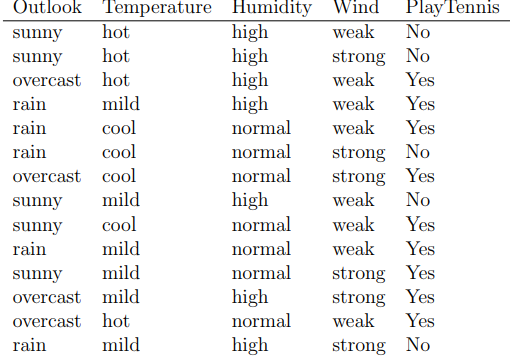
\includegraphics{1.png}
\caption{}
\end{figure}

    \subsubsection*{Root Node}\label{root-node}

    First construct a few tables for each attribute to \textbf{entropy} and
\textbf{info gain} calculation:

\begin{figure}[H]
\centering
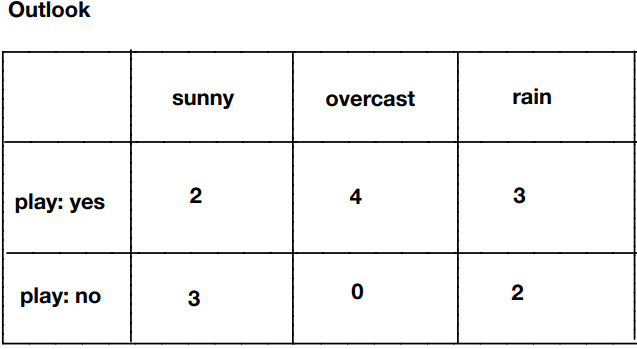
\includegraphics{3.png}
\caption{}
\end{figure}

\begin{figure}[H]
\centering
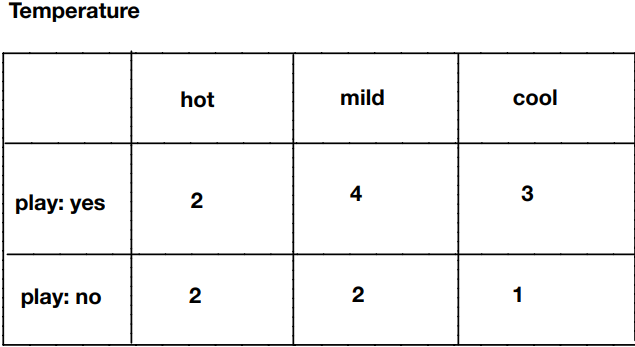
\includegraphics{4.png}
\caption{}
\end{figure}

\begin{figure}[H]
\centering
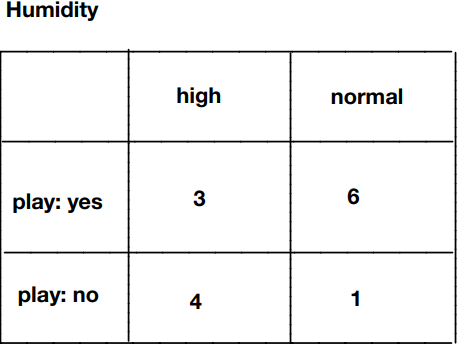
\includegraphics{5.png}
\caption{}
\end{figure}

\begin{figure}[H]
\centering
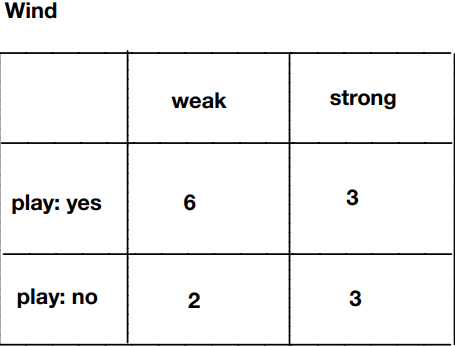
\includegraphics{6.png}
\caption{}
\end{figure}

Entropy before split:

\[E = -\frac{9}{14} \log (\frac{9}{14}) -  \frac{9}{14} \log (\frac{9}{14}) = 0.940\]

\begin{itemize}
\tightlist
\item
  Entropy after splitting on \emph{Outlook}:
\end{itemize}

\[E(Outlook_{sunny}) = -\frac{2}{5} \log \frac{2}{5} - \frac{3}{5} \log \frac{2}{5} = 0.971\]

\[E(Outlook_{overcast}) = - \frac{4}{4} \log \frac{4}{4} = 0 \]

\[E(Outlook_{rain}) = -\frac{2}{5} \log \frac{2}{5} - \frac{3}{5} \log \frac{2}{5} = 0.971\]

\[\text{ Info gain }(Outlook)= E - \frac{5}{14} E(Outlook_{sunny}) - \frac{4}{14} E(Outlook_{overcast}) - - \frac{5}{14} E(Outlook_{rain})  = 0.940 - \frac{5}{14} \cdot 0.971 \cdot 2  = 0.246\]

\begin{itemize}
\tightlist
\item
  Entropy after splitting on \emph{Temperature}:
\end{itemize}

\[E(Temperature_{hot}) = -\frac{2}{4} \log \frac{2}{4} \cdot 2 = 1\]

\[E(Temperature_{mild})= - \frac{4}{6} \log \frac{4}{6} - \frac{2}{6} \log \frac{2}{6} = 0.918\]

\[E(Temperature_{cool})= - \frac{3}{4} \log \frac{3}{4} - \frac{1}{4} \log \frac{1}{4} = 0.811\]

\[\text{Info gain}(Temperature) = E - \frac{4}{14} E(Temperature_{hot}) - \frac{6}{14}E(Temperature_{mild}) - \frac{4}{14}E(Temperature_{cool}) \]

\[ = 0.940 - \frac{4}{14} \cdot 1 - \frac{6}{14} \cdot 0.918 - \frac{4}{14} \cdot 0.811 = 0.029\]

\begin{itemize}
\tightlist
\item
  Entropy after splitting on \emph{Humidity}:
\end{itemize}

\[E(Humidity_{high}) = -\frac{3}{7} \log \frac{3}{7} - \frac{4}{7} \log \frac{4}{7} = 0.985\]

\[E(Humidity_{normal}) = -\frac{6}{7} \log \frac{6}{7} - \frac{1}{7} \log \frac{1}{7}= 0.592\]

\[\text{ Info gain }(Humidity)= E - \frac{7}{14} E(Humidity_{high}) - \frac{7}{14} E(Humidity_{normal})  = 0.940 - \frac{7}{14} \cdot 0.985 -  \frac{7}{14} \cdot 0.592  = 0.152\]

\begin{itemize}
\tightlist
\item
  Entropy after splitting on \emph{Wind}:
\end{itemize}

\[E(Wind_{weak}) = -\frac{6}{8} \log \frac{6}{8} - \frac{2}{8} \log \frac{2}{8} = 0.811\]

\[E(Wind_{strong}) = -\frac{3}{6} \log \frac{3}{6}  \cdot 2= 1\]

\[\text{ Info gain }(Wind)= E - \frac{8}{14} E(Wind_{weak})  - \frac{6}{14} E(Wind_{strong}) = 0.940 - \frac{8}{14} \cdot 0.811 -  \frac{6}{14} \cdot 1  = 0.048\]

Since
\(info \: gain(Outlook) = 0.246 > info \: gain(Humidity) = 0.152> info \: gain(Wind) = 0.048> info \: gain(Temperature) = 0.029\),
so if split on \emph{Outlook}, the reduction of entropy, i.e. the
reduction of uncertainty is larger than splitting on others. Thus
\textbf{Outlook} should be selected for the root node for the
Decision Tree.

    \subsubsection*{First Child}\label{first-child}

    Since \(Outlook_{overcast}\) is pure, thus no further split is required.
Hence next split should be on \(Outlook_{sunny}\) and \(Outlook_{rain}\)

\begin{itemize}
\tightlist
\item
  Outlook:sunny
\end{itemize}

\begin{figure}[H]
\centering
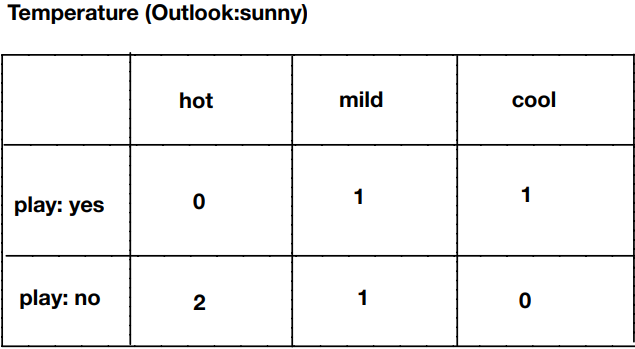
\includegraphics{7.png}
\caption{}
\end{figure}

\begin{figure}[H]
\centering
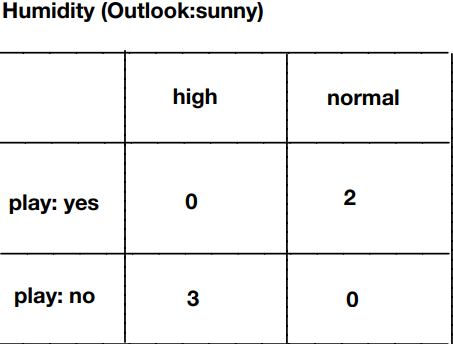
\includegraphics{8.png}
\caption{}
\end{figure}

\begin{figure}[H]
\centering
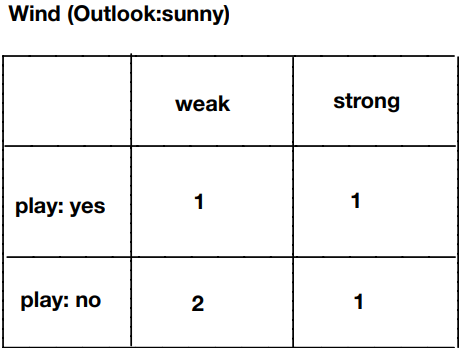
\includegraphics{9.png}
\caption{}
\end{figure}

Entropy before split:

\[E = -\frac{2}{5} \log (\frac{2}{5}) -  \frac{3}{5} \log (\frac{3}{5}) = 0.971\]

\begin{itemize}
\tightlist
\item
  Entropy after splitting on \emph{Temperature}:
\end{itemize}

\[E(Temperature_{hot}) = 0\]

\[E(Temperature_{mild})= 1 = 0.918\]

\[E(Temperature_{cool})= 0 \]

\[\text{Info gain}(Temperature) = E - \frac{2}{5} E(Temperature_{hot}) - \frac{2}{5}E(Temperature_{mild}) - \frac{1}{5}E(Temperature_{cool})  = 0.971 - 0.4= 0.571\]

\begin{itemize}
\tightlist
\item
  Entropy after splitting on \emph{Humidity}:
\end{itemize}

\[E(Humidity_{high}) = 0\]

\[E(Humidity_{normal}) = 0\]

\[\text{ Info gain }(Humidity)= E = 0.971\]

\begin{itemize}
\tightlist
\item
  Entropy after splitting on \emph{Wind}:
\end{itemize}

\[E(Wind_{weak}) = -\frac{1}{3} \log \frac{1}{3} - \frac{2}{3} \log \frac{2}{3} = 0.918\]

\[E(Wind_{strong}) = 1\]

\[\text{ Info gain }(Wind)= E - \frac{3}{5} E(Wind_{weak})  - \frac{2}{5} E(Wind_{strong}) = 0.971 - 0.6 \cdot 0.918 -  0.4 \cdot 1  = 0.0202\]

Since
\(info \: gain(Humidity) = 0.971> info \: gain(Temperature) = 0.571> info \: gain(Wind) = 0.0201\),
so if split on \emph{Humidity}, the reduction of entropy, i.e. the
reduction of uncertainty is larger than splitting on others. Thus
\textbf{Humidity} should be selected for the next node for the
Decision Tree.

\begin{itemize}
\tightlist
\item
  Outlook:rain
\end{itemize}

\begin{figure}[H]
\centering

\includegraphics{10.png}
\caption{}
\end{figure}

\begin{figure}[H]
\centering
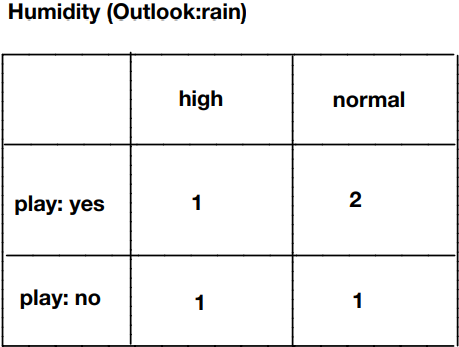
\includegraphics{11.png}
\caption{}
\end{figure}

\begin{figure}[H]
\centering
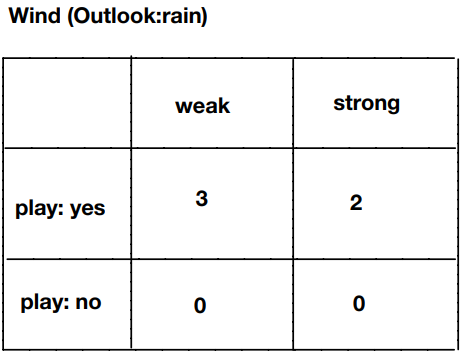
\includegraphics{12.png}
\caption{}
\end{figure}

Entropy before split:

\[E = -\frac{2}{5} \log (\frac{2}{5}) -  \frac{3}{5} \log (\frac{3}{5}) = 0.971\]

\begin{itemize}
\tightlist
\item
  Entropy after splitting on \emph{Temperature}:
\end{itemize}

\[E(Temperature_{mild})= -\frac{1}{3} \log \frac{1}{3} - \frac{2}{3} \log \frac{2}{3} = 0.918\]

\[E(Temperature_{cool})= 1 \]

\[\text{Info gain}(Temperature) = E -  \frac{3}{5}E(Temperature_{mild}) - \frac{2}{5}E(Temperature_{cool})  = 0.971 - 0.6 \cdot 0.918 - 0.4 \cdot 1 = 0.0202\]

\begin{itemize}
\tightlist
\item
  Entropy after splitting on \emph{Humidity}:
\end{itemize}

\[E(Humidity_{high}) = 1\]

\[E(Humidity_{normal}) = -\frac{1}{3} \log \frac{1}{3} - \frac{2}{3} \log \frac{2}{3} = 0.918\]

\[\text{ Info gain }(Humidity)= E -  \frac{2}{5}E(Humidity_{high})) - \frac{3}{5}E(Humidity_{normal})  = 0.971 - 0.6 \cdot 0.918 - 0.4 \cdot 1 = 0.0202\]

\begin{itemize}
\tightlist
\item
  Entropy after splitting on \emph{Wind}:
\end{itemize}

\[E(Wind_{weak}) = 0\]

\[E(Wind_{strong}) = 0\]

\[\text{ Info gain }(Wind)= E  = 0.971\]

Since
\(info \: gain(Wind) = 0.971> info \: gain(Temperature) = 0.0202= info \: gain(Humidity) = 0.0202\),
so if split on \emph{Wind}, the reduction of entropy, i.e. the reduction
of uncertainty is larger than splitting on others. Thus
\textbf{Wind} should be selected for the next node for the
Decision Tree.\\

    Till this point, there's no impure attribute that needed to be splitted.
Therefore, the Decision Tree construction is completed.

\subsubsection*{Final Tree:}\label{final-tree}

\begin{figure}[H]
\centering
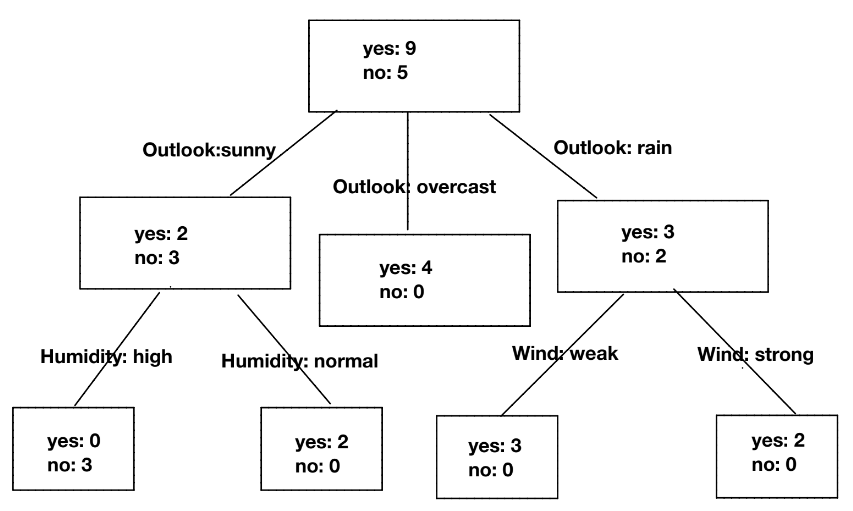
\includegraphics{13.png}
\caption{}
\end{figure}

    \subsubsection*{Q3}\label{q3}

    3.(25 pts.) Recall the use of bag of words representation for text
classification. Note that in a bag of words representation each document
is encoded using a bag of words. Consider a more general scenario in
which it might be beneficial to encode a data sample to be classified
using multiple bags of features that correspond to perhaps different
modality (e.g., textual features or words, visual features, etc. in the
case of a document that contains both words and pictures). We can think
of each modality as being associated with its own vocabulary (e.g., a
set of words, a set of visual features, etc.). Precisely formulate the
problem of learning classifiers in a setting wherein each data sample is
represented using multiple (say M) bags of features, one for each
modality. Outline a learning algorithm (at sufficient detail needed for
implementation). Hint: You may consider variations or adaptations of the
learning algorithms that you have studied so far\\\\


\textbf{Answer:}


    This should probably considered as a MultiModality Learning
problem, in which different format of data sources, like images, texts,
videos, audios are used together to extract features from each and
concatenate with data fusion techniques for a machine learning task,
examples I know are mostly in the field of computer vision, such as
image captioning, context encoder for task like image inpainting,
semantic image segmentation, etc. In this case, the task is text
classification, and major data formats include text and images. Thus a
possible algorithm pipeline could be constructed as follows:

\begin{itemize}
\tightlist
\item
  Data Preprocessing

  \begin{itemize}
  \tightlist
  \item
    Feature Engineering

    \begin{itemize}
    \tightlist
    \item
      text

      \begin{itemize}
      \tightlist
      \item
        BOW
      \item
        TF-IDF
      \item
        Word2Vec
      \end{itemize}
    \item
      image

      \begin{itemize}
      \tightlist
      \item
        BOVW (Bag of Visual Words, inspired by BOW)

        eg: SIFT/ORB/SURF
      \end{itemize}
    \end{itemize}
  \item
    Feature Fusion
  \end{itemize}
\item
  Classifier

  \begin{itemize}
  \tightlist
  \item
    Naive Bayes
  \item
    Decision Tree
  \item
    Logistic Regression
  \item
    ...
  \end{itemize}
\end{itemize}

    \subsubsection*{Example (because I could not find a dataset for document
classification task that includes both text and images ready to train,
so the code is a just general idea of what I think how the algorithm probably
works):}\label{example-because-i-could-not-find-a-dataset-for-document-classification-task-that-includes-both-text-and-images-ready-to-train-so-the-code-is-a-general-idea-of-what-i-think-how-the-algorithm-probably-works}

    \begin{Verbatim}[commandchars=\\\{\}]
{\color{incolor}In [{\color{incolor}11}]:} \PY{k+kn}{from} \PY{n+nn}{sklearn}\PY{n+nn}{.}\PY{n+nn}{datasets} \PY{k}{import} \PY{n}{fetch\PYZus{}20newsgroups} \PY{c+c1}{\PYZsh{} just a random example}
         \PY{k+kn}{from} \PY{n+nn}{sklearn}\PY{n+nn}{.}\PY{n+nn}{feature\PYZus{}extraction}\PY{n+nn}{.}\PY{n+nn}{text} \PY{k}{import} \PY{n}{CountVectorizer}\PY{p}{,} \PY{n}{TfidfVectorizer}
         \PY{k+kn}{from} \PY{n+nn}{sklearn}\PY{n+nn}{.}\PY{n+nn}{naive\PYZus{}bayes} \PY{k}{import} \PY{n}{GaussianNB}
         \PY{k+kn}{from} \PY{n+nn}{sklearn}\PY{n+nn}{.}\PY{n+nn}{tree} \PY{k}{import} \PY{n}{DecisionTreeClassifier}
         \PY{k+kn}{from} \PY{n+nn}{sklearn}\PY{n+nn}{.}\PY{n+nn}{ensemble} \PY{k}{import} \PY{n}{RandomForestClassifier}\PY{p}{,} 
         \PY{k+kn}{from} \PY{n+nn}{sklearn}\PY{n+nn}{.}\PY{n+nn}{linear\PYZus{}model} \PY{k}{import} \PY{n}{LogisticRegression}
         \PY{k+kn}{from} \PY{n+nn}{sklearn}\PY{n+nn}{.}\PY{n+nn}{neural\PYZus{}network} \PY{k}{import} \PY{n}{MLPClassifier} 
         \PY{k+kn}{from} \PY{n+nn}{sklearn}\PY{n+nn}{.}\PY{n+nn}{preprocessing} \PY{k}{import} \PY{n}{StandardScaler}
         \PY{k+kn}{from} \PY{n+nn}{scipy}\PY{n+nn}{.}\PY{n+nn}{cluster} \PY{k}{import} \PY{n}{vq}
         \PY{k+kn}{from} \PY{n+nn}{sklearn}\PY{n+nn}{.}\PY{n+nn}{cluster} \PY{k}{import} \PY{n}{KMeans}
         \PY{k+kn}{import} \PY{n+nn}{matplotlib}\PY{n+nn}{.}\PY{n+nn}{pyplot} \PY{k}{as} \PY{n+nn}{plt}
         \PY{k+kn}{import} \PY{n+nn}{cv2}
         \PY{k+kn}{import} \PY{n+nn}{glob}
         \PY{k+kn}{import} \PY{n+nn}{pandas} \PY{k}{as} \PY{n+nn}{pd}
         \PY{k+kn}{import} \PY{n+nn}{numpy} \PY{k}{as} \PY{n+nn}{np}
         \PY{k+kn}{import} \PY{n+nn}{nltk}
         \PY{k+kn}{import} \PY{n+nn}{gensim}
         
         
         \PY{c+c1}{\PYZsh{} just a random example (the image dataset and text dataset have no relations)}
         \PY{n}{IMAGENET\PYZus{}CAR} \PY{o}{=} \PY{l+s+s1}{\PYZsq{}}\PY{l+s+s1}{/home/karen/Downloads/data/ImageNet\PYZus{}Utils/imageNet\PYZus{}dataset/train/car}\PY{l+s+s1}{\PYZsq{}}
         
         
         \PY{k}{class} \PY{n+nc}{MultuModalityPipeline}\PY{p}{:}
             
             \PY{k}{def} \PY{n+nf}{\PYZus{}\PYZus{}init\PYZus{}\PYZus{}}\PY{p}{(}\PY{n+nb+bp}{self}\PY{p}{)}\PY{p}{:}
                 \PY{n+nb+bp}{self}\PY{o}{.}\PY{n}{text\PYZus{}dataset} \PY{o}{=} \PY{n}{fetch\PYZus{}20newsgroups}\PY{p}{(}\PY{n}{subset}\PY{o}{=}\PY{l+s+s1}{\PYZsq{}}\PY{l+s+s1}{train}\PY{l+s+s1}{\PYZsq{}}\PY{p}{,} \PY{n}{shuffle}\PY{o}{=}\PY{k+kc}{True}\PY{p}{)}
                 \PY{c+c1}{\PYZsh{} pick the top 20 as an example to see what the result will be like}
                 \PY{n+nb+bp}{self}\PY{o}{.}\PY{n}{text\PYZus{}X} \PY{o}{=} \PY{n+nb+bp}{self}\PY{o}{.}\PY{n}{text\PYZus{}dataset}\PY{o}{.}\PY{n}{data}\PY{p}{[}\PY{p}{:}\PY{l+m+mi}{20}\PY{p}{]}
                 \PY{n+nb+bp}{self}\PY{o}{.}\PY{n}{text\PYZus{}y} \PY{o}{=} \PY{n+nb+bp}{self}\PY{o}{.}\PY{n}{text\PYZus{}dataset}\PY{o}{.}\PY{n}{target}\PY{p}{[}\PY{p}{:}\PY{l+m+mi}{20}\PY{p}{]}
                 \PY{n+nb+bp}{self}\PY{o}{.}\PY{n}{image\PYZus{}dataset} \PY{o}{=} \PY{n}{glob}\PY{o}{.}\PY{n}{glob}\PY{p}{(}\PY{l+s+s2}{\PYZdq{}}\PY{l+s+si}{\PYZpc{}s}\PY{l+s+s2}{/*}\PY{l+s+s2}{\PYZdq{}} \PY{o}{\PYZpc{}}\PY{k}{IMAGENET\PYZus{}CAR})[:20]
                 
             \PY{k}{def} \PY{n+nf}{create\PYZus{}word2vec\PYZus{}matrix}\PY{p}{(}\PY{n+nb+bp}{self}\PY{p}{,} \PY{n}{text}\PY{p}{,} \PY{n}{word2vec}\PY{p}{)}\PY{p}{:}
                 \PY{n}{word2vec\PYZus{}matrix}\PY{o}{=}\PY{p}{[}\PY{p}{]}
                 \PY{k}{for} \PY{n}{idx}\PY{p}{,} \PY{n}{line} \PY{o+ow}{in} \PY{n+nb}{enumerate}\PY{p}{(}\PY{n}{text}\PY{p}{)}\PY{p}{:}
                     \PY{n}{regex} \PY{o}{=} \PY{n}{nltk}\PY{o}{.}\PY{n}{tokenize}\PY{o}{.}\PY{n}{RegexpTokenizer}\PY{p}{(}\PY{l+s+sa}{r}\PY{l+s+s1}{\PYZsq{}}\PY{l+s+s1}{[a\PYZhy{}zA\PYZhy{}Z]+}\PY{l+s+s1}{\PYZsq{}}\PY{p}{)}
                     \PY{n}{word\PYZus{}lst} \PY{o}{=} \PY{l+s+s1}{\PYZsq{}}\PY{l+s+s1}{ }\PY{l+s+s1}{\PYZsq{}}\PY{o}{.}\PY{n}{join}\PY{p}{(}\PY{n}{regex}\PY{o}{.}\PY{n}{tokenize}\PY{p}{(}\PY{n}{line}\PY{p}{)}\PY{p}{)}
                     \PY{n}{current\PYZus{}word2vec}\PY{o}{=}\PY{p}{[}\PY{p}{]}
                     \PY{k}{for} \PY{n}{word} \PY{o+ow}{in} \PY{n}{word\PYZus{}lst}\PY{p}{:}
                         \PY{k}{if} \PY{n}{word} \PY{o+ow}{in} \PY{n}{word2vec}\PY{o}{.}\PY{n}{vocab}\PY{p}{:}
                             \PY{n}{vec} \PY{o}{=} \PY{n}{word2vec}\PY{o}{.}\PY{n}{vectors\PYZus{}norm}\PY{p}{[}\PY{n}{word2vec}\PY{o}{.}\PY{n}{vocab}\PY{p}{[}\PY{n}{word}\PY{p}{]}\PY{o}{.}\PY{n}{index}\PY{p}{]}
                             \PY{k}{if} \PY{n}{vec} \PY{o+ow}{is} \PY{o+ow}{not} \PY{k+kc}{None}\PY{p}{:}
                                 \PY{n}{current\PYZus{}word2vec}\PY{o}{.}\PY{n}{append}\PY{p}{(}\PY{n}{vec}\PY{p}{)}
                     \PY{k}{if} \PY{n}{np}\PY{o}{.}\PY{n}{array}\PY{p}{(}\PY{n}{current\PYZus{}word2vec}\PY{p}{)}\PY{o}{.}\PY{n}{shape}\PY{p}{[}\PY{l+m+mi}{0}\PY{p}{]}\PY{o}{!=}\PY{l+m+mi}{0}\PY{p}{:}
                         \PY{n}{sentence\PYZus{}word2vec} \PY{o}{=} \PY{n+nb}{list}\PY{p}{(}\PY{n}{np}\PY{o}{.}\PY{n}{array}\PY{p}{(}\PY{n}{current\PYZus{}word2vec}\PY{p}{)}\PY{o}{.}\PY{n}{mean}\PY{p}{(}\PY{n}{axis}\PY{o}{=}\PY{l+m+mi}{0}\PY{p}{)}\PY{p}{)}
                         \PY{n}{word2vec\PYZus{}matrix}\PY{o}{.}\PY{n}{append}\PY{p}{(}\PY{n}{sentence\PYZus{}word2vec}\PY{p}{)}
                     \PY{n}{current\PYZus{}word2vec}\PY{o}{=}\PY{p}{[}\PY{p}{]}
                 \PY{k}{return} \PY{n}{word2vec\PYZus{}matrix}
                 
         
             \PY{k}{def} \PY{n+nf}{word\PYZus{}feature\PYZus{}vectorizer}\PY{p}{(}\PY{n+nb+bp}{self}\PY{p}{,} \PY{n}{option} \PY{o}{=} \PY{l+s+s1}{\PYZsq{}}\PY{l+s+s1}{BOW}\PY{l+s+s1}{\PYZsq{}}\PY{p}{)}\PY{p}{:}
                 \PY{k}{if} \PY{n}{option} \PY{o}{!=} \PY{l+s+s1}{\PYZsq{}}\PY{l+s+s1}{Word2Vec}\PY{l+s+s1}{\PYZsq{}}\PY{p}{:}
                     \PY{k}{if} \PY{n}{option} \PY{o}{==} \PY{l+s+s1}{\PYZsq{}}\PY{l+s+s1}{BOW}\PY{l+s+s1}{\PYZsq{}}\PY{p}{:}
                         \PY{c+c1}{\PYZsh{} n\PYZhy{}gram = 1 ~ 2}
                         \PY{n}{vect} \PY{o}{=} \PY{n}{CountVectorizer}\PY{p}{(}\PY{n}{token\PYZus{}pattern}\PY{o}{=}\PY{l+s+s1}{\PYZsq{}}\PY{l+s+s1}{[a\PYZhy{}zA\PYZhy{}Z]+}\PY{l+s+s1}{\PYZsq{}}\PY{p}{,} \PY{n}{ngram\PYZus{}range}\PY{o}{=}\PY{p}{(}\PY{p}{[}\PY{l+m+mi}{1}\PY{p}{,}\PY{l+m+mi}{2}\PY{p}{]}\PY{p}{)}\PY{p}{,} 
                             \PY{n}{preprocessor}\PY{o}{=}\PY{k+kc}{None}\PY{p}{,} \PY{n}{stop\PYZus{}words}\PY{o}{=}\PY{l+s+s1}{\PYZsq{}}\PY{l+s+s1}{english}\PY{l+s+s1}{\PYZsq{}}\PY{p}{,} \PY{n}{max\PYZus{}features}\PY{o}{=}\PY{l+m+mi}{3000}\PY{p}{)}
                     \PY{k}{elif} \PY{n}{option} \PY{o}{==} \PY{l+s+s1}{\PYZsq{}}\PY{l+s+s1}{TFIDF}\PY{l+s+s1}{\PYZsq{}}\PY{p}{:}
                         \PY{n}{vect} \PY{o}{=} \PY{n}{TfidfVectorizer}\PY{p}{(}\PY{n}{token\PYZus{}pattern}\PY{o}{=}\PY{l+s+s1}{\PYZsq{}}\PY{l+s+s1}{[a\PYZhy{}zA\PYZhy{}Z]+}\PY{l+s+s1}{\PYZsq{}}\PY{p}{,} \PY{n}{analyzer} \PY{o}{=} \PY{l+s+s1}{\PYZsq{}}\PY{l+s+s1}{word}\PY{l+s+s1}{\PYZsq{}}\PY{p}{,} 
                         \PY{n}{sublinear\PYZus{}tf}\PY{o}{=}\PY{k+kc}{True}\PY{p}{,} \PY{n}{min\PYZus{}df}\PY{o}{=}\PY{l+m+mi}{10}\PY{p}{,} \PY{n}{norm}\PY{o}{=}\PY{l+s+s1}{\PYZsq{}}\PY{l+s+s1}{l1}\PY{l+s+s1}{\PYZsq{}}\PY{p}{,} \PY{n}{encoding}\PY{o}{=}\PY{l+s+s1}{\PYZsq{}}\PY{l+s+s1}{latin\PYZhy{}1}\PY{l+s+s1}{\PYZsq{}}\PY{p}{,} 
                                                     \PY{n}{ngram\PYZus{}range}\PY{o}{=}\PY{p}{(}\PY{l+m+mi}{1}\PY{p}{,}\PY{l+m+mi}{2}\PY{p}{)}\PY{p}{,} \PY{n}{stop\PYZus{}words}\PY{o}{=}\PY{l+s+s1}{\PYZsq{}}\PY{l+s+s1}{english}\PY{l+s+s1}{\PYZsq{}}\PY{p}{)}
         
                     \PY{n}{X\PYZus{}vect} \PY{o}{=} \PY{n}{vect}\PY{o}{.}\PY{n}{fit\PYZus{}transform}\PY{p}{(}\PY{n+nb+bp}{self}\PY{o}{.}\PY{n}{text\PYZus{}X}\PY{p}{)}
                     \PY{k}{return} \PY{n}{X\PYZus{}vect}\PY{p}{,} \PY{n}{vect}\PY{o}{.}\PY{n}{get\PYZus{}feature\PYZus{}names}\PY{p}{(}\PY{p}{)}
                 \PY{k}{else}\PY{p}{:}
                     \PY{n}{wv} \PY{o}{=} \PY{n}{gensim}\PY{o}{.}\PY{n}{models}\PY{o}{.}\PY{n}{KeyedVectors}\PY{o}{.}\PY{n}{load\PYZus{}word2vec\PYZus{}format}\PY{p}{(}\PY{n}{fname}\PY{o}{=}
                     \PY{l+s+s1}{\PYZsq{}}\PY{l+s+s1}{/home/karen/Downloads/data/GoogleNews\PYZhy{}vectors\PYZhy{}negative300.bin.gz}\PY{l+s+s1}{\PYZsq{}}\PY{p}{,} 
                                                              \PY{n}{binary}\PY{o}{=}\PY{k+kc}{True}\PY{p}{)}
                     \PY{n}{wv}\PY{o}{.}\PY{n}{init\PYZus{}sims}\PY{p}{(}\PY{n}{replace}\PY{o}{=}\PY{k+kc}{True}\PY{p}{)}
                     \PY{n}{wv\PYZus{}matrix} \PY{o}{=} \PY{n+nb+bp}{self}\PY{o}{.}\PY{n}{create\PYZus{}word2vec\PYZus{}matrix}\PY{p}{(}\PY{n}{text}\PY{o}{=}\PY{n+nb+bp}{self}\PY{o}{.}\PY{n}{text\PYZus{}X}\PY{p}{,} \PY{n}{word2vec}\PY{o}{=}\PY{n}{wv}\PY{p}{)}
                     \PY{k}{return} \PY{n}{wv\PYZus{}matrix}
                     
             
             \PY{k}{def} \PY{n+nf}{img\PYZus{}feature\PYZus{}vectorizer}\PY{p}{(}\PY{n+nb+bp}{self}\PY{p}{,} \PY{n}{num\PYZus{}features}\PY{p}{,} \PY{n}{option} \PY{o}{=} \PY{l+s+s1}{\PYZsq{}}\PY{l+s+s1}{ORB}\PY{l+s+s1}{\PYZsq{}}\PY{p}{)}\PY{p}{:}
                 \PY{n}{dataset\PYZus{}size} \PY{o}{=} \PY{n+nb}{len}\PY{p}{(}\PY{n+nb+bp}{self}\PY{o}{.}\PY{n}{image\PYZus{}dataset}\PY{p}{)}
                 \PY{n}{resp} \PY{o}{=} \PY{n}{np}\PY{o}{.}\PY{n}{zeros}\PY{p}{(}\PY{p}{(}\PY{n}{dataset\PYZus{}size}\PY{p}{,} \PY{l+m+mi}{1}\PY{p}{)}\PY{p}{)}
                 \PY{n}{des\PYZus{}list} \PY{o}{=} \PY{p}{[}\PY{p}{]}
                 \PY{k}{for} \PY{n}{idx}\PY{p}{,} \PY{n}{f} \PY{o+ow}{in} \PY{n+nb}{enumerate}\PY{p}{(}\PY{n+nb+bp}{self}\PY{o}{.}\PY{n}{image\PYZus{}dataset}\PY{p}{)}\PY{p}{:}
                     \PY{n}{img} \PY{o}{=} \PY{n}{cv2}\PY{o}{.}\PY{n}{imread}\PY{p}{(}\PY{n}{f}\PY{p}{)}
                     \PY{n}{img} \PY{o}{=} \PY{n}{cv2}\PY{o}{.}\PY{n}{cvtColor}\PY{p}{(}\PY{n}{img}\PY{p}{,} \PY{n}{cv2}\PY{o}{.}\PY{n}{COLOR\PYZus{}BGR2RGB}\PY{p}{)}
                     \PY{k}{if} \PY{n}{option} \PY{o}{==} \PY{l+s+s1}{\PYZsq{}}\PY{l+s+s1}{ORB}\PY{l+s+s1}{\PYZsq{}}\PY{p}{:}
                         \PY{n}{descriptor} \PY{o}{=} \PY{n}{cv2}\PY{o}{.}\PY{n}{ORB\PYZus{}create}\PY{p}{(}\PY{p}{)}
                     \PY{k}{elif} \PY{n}{option} \PY{o}{==} \PY{l+s+s1}{\PYZsq{}}\PY{l+s+s1}{SIFT}\PY{l+s+s1}{\PYZsq{}}\PY{p}{:}
                         \PY{n}{descriptor} \PY{o}{=} \PY{n}{cv2}\PY{o}{.}\PY{n}{xfeatures2d}\PY{o}{.}\PY{n}{SIFT\PYZus{}create}\PY{p}{(}\PY{p}{)}
                     \PY{k}{elif} \PY{n}{option} \PY{o}{==} \PY{l+s+s1}{\PYZsq{}}\PY{l+s+s1}{SURF}\PY{l+s+s1}{\PYZsq{}}\PY{p}{:}
                         \PY{n}{descriptor} \PY{o}{=} \PY{n}{cv2}\PY{o}{.}\PY{n}{xfeatures2d}\PY{o}{.}\PY{n}{SURF\PYZus{}create}\PY{p}{(}\PY{p}{)}
                     
                     \PY{p}{(}\PY{n}{\PYZus{}}\PY{p}{,} \PY{n}{features}\PY{p}{)} \PY{o}{=} \PY{n}{descriptor}\PY{o}{.}\PY{n}{detectAndCompute}\PY{p}{(}\PY{n}{img}\PY{p}{,} \PY{k+kc}{None}\PY{p}{)}
                     \PY{n}{des} \PY{o}{=} \PY{n}{np}\PY{o}{.}\PY{n}{float32}\PY{p}{(}\PY{n}{features}\PY{p}{)}
                     \PY{n}{des\PYZus{}list}\PY{o}{.}\PY{n}{append}\PY{p}{(}\PY{p}{(}\PY{n}{f}\PY{p}{,} \PY{n}{des}\PY{p}{)}\PY{p}{)}
         
                 \PY{n}{descriptors} \PY{o}{=} \PY{n}{des\PYZus{}list}\PY{p}{[}\PY{l+m+mi}{0}\PY{p}{]}\PY{p}{[}\PY{l+m+mi}{1}\PY{p}{]}
                 \PY{k}{for} \PY{n}{image\PYZus{}path}\PY{p}{,} \PY{n}{descriptor} \PY{o+ow}{in} \PY{n}{des\PYZus{}list}\PY{p}{[}\PY{l+m+mi}{1}\PY{p}{:}\PY{p}{]}\PY{p}{:}
                     \PY{n}{descriptors} \PY{o}{=} \PY{n}{np}\PY{o}{.}\PY{n}{vstack}\PY{p}{(}\PY{p}{(}\PY{n}{descriptors}\PY{p}{,} \PY{n}{descriptor}\PY{p}{)}\PY{p}{)}
         
                 \PY{n}{criteria} \PY{o}{=} \PY{p}{(}\PY{n}{cv2}\PY{o}{.}\PY{n}{TERM\PYZus{}CRITERIA\PYZus{}EPS} \PY{o}{+} \PY{n}{cv2}\PY{o}{.}\PY{n}{TERM\PYZus{}CRITERIA\PYZus{}MAX\PYZus{}ITER}\PY{p}{,} \PY{l+m+mi}{10}\PY{p}{,} \PY{l+m+mf}{1.0}\PY{p}{)}
                 \PY{n}{flags} \PY{o}{=} \PY{n}{cv2}\PY{o}{.}\PY{n}{KMEANS\PYZus{}RANDOM\PYZus{}CENTERS}
                 \PY{n+nb}{print}\PY{p}{(}\PY{n}{descriptors}\PY{o}{.}\PY{n}{shape}\PY{p}{)}
                 \PY{n}{\PYZus{}}\PY{p}{,} \PY{n}{\PYZus{}}\PY{p}{,} \PY{n}{centers} \PY{o}{=} \PY{n}{cv2}\PY{o}{.}\PY{n}{kmeans}\PY{p}{(}\PY{n}{descriptors}\PY{p}{,} \PY{n}{num\PYZus{}features}\PY{p}{,} \PY{k+kc}{None}\PY{p}{,} \PY{n}{criteria}\PY{p}{,} \PY{l+m+mi}{10}\PY{p}{,} \PY{n}{flags}\PY{p}{)}
                 \PY{n}{im\PYZus{}features} \PY{o}{=} \PY{n}{np}\PY{o}{.}\PY{n}{zeros}\PY{p}{(}\PY{p}{(}\PY{n}{dataset\PYZus{}size}\PY{p}{,} \PY{n}{num\PYZus{}features}\PY{p}{)}\PY{p}{,} \PY{l+s+s2}{\PYZdq{}}\PY{l+s+s2}{float32}\PY{l+s+s2}{\PYZdq{}}\PY{p}{)}
                 \PY{k}{for} \PY{n}{i} \PY{o+ow}{in} \PY{n+nb}{range}\PY{p}{(}\PY{n}{dataset\PYZus{}size}\PY{p}{)}\PY{p}{:}
                     \PY{n}{words}\PY{p}{,} \PY{n}{distance} \PY{o}{=} \PY{n}{vq}\PY{o}{.}\PY{n}{vq}\PY{p}{(}\PY{n}{des\PYZus{}list}\PY{p}{[}\PY{n}{i}\PY{p}{]}\PY{p}{[}\PY{l+m+mi}{1}\PY{p}{]}\PY{p}{,} \PY{n}{centers}\PY{p}{)}
                     \PY{k}{for} \PY{n}{w} \PY{o+ow}{in} \PY{n}{words}\PY{p}{:}
                         \PY{n}{im\PYZus{}features}\PY{p}{[}\PY{n}{i}\PY{p}{]}\PY{p}{[}\PY{n}{w}\PY{p}{]} \PY{o}{+}\PY{o}{=} \PY{l+m+mi}{1}
         
                 \PY{c+c1}{\PYZsh{} Scaling the values of features}
                 \PY{n}{im\PYZus{}features} \PY{o}{=} \PY{n}{StandardScaler}\PY{p}{(}\PY{p}{)}\PY{o}{.}\PY{n}{fit}\PY{p}{(}\PY{n}{im\PYZus{}features}\PY{p}{)}\PY{o}{.}\PY{n}{transform}\PY{p}{(}\PY{n}{im\PYZus{}features}\PY{p}{)}
         
                 \PY{k}{return} \PY{n}{im\PYZus{}features}
         
         
             \PY{k}{def} \PY{n+nf}{classifier}\PY{p}{(}\PY{n+nb+bp}{self}\PY{p}{,} \PY{n}{option}\PY{o}{=}\PY{l+s+s1}{\PYZsq{}}\PY{l+s+s1}{NB}\PY{l+s+s1}{\PYZsq{}}\PY{p}{)}\PY{p}{:}
                 \PY{k}{if} \PY{n}{option} \PY{o}{==} \PY{l+s+s1}{\PYZsq{}}\PY{l+s+s1}{NB}\PY{l+s+s1}{\PYZsq{}}\PY{p}{:}
                     \PY{n}{clf} \PY{o}{=} \PY{n}{GaussianNB}\PY{p}{(}\PY{p}{)}
                 \PY{k}{elif} \PY{n}{option} \PY{o}{==} \PY{l+s+s1}{\PYZsq{}}\PY{l+s+s1}{DT}\PY{l+s+s1}{\PYZsq{}}\PY{p}{:}
                     \PY{n}{clf} \PY{o}{=} \PY{n}{DecisionTreeClassifier}\PY{p}{(}\PY{n}{criterion} \PY{o}{=} \PY{l+s+s1}{\PYZsq{}}\PY{l+s+s1}{entropy}\PY{l+s+s1}{\PYZsq{}}\PY{p}{,}
                                                     \PY{n}{random\PYZus{}state} \PY{o}{=} \PY{l+m+mi}{100}\PY{p}{,}
                                                     \PY{n}{max\PYZus{}depth} \PY{o}{=} \PY{l+m+mi}{5}\PY{p}{,}
                                                     \PY{n}{min\PYZus{}samples\PYZus{}leaf} \PY{o}{=} \PY{l+m+mi}{2}\PY{p}{)}
                 \PY{k}{elif} \PY{n}{option} \PY{o}{==} \PY{l+s+s1}{\PYZsq{}}\PY{l+s+s1}{RF}\PY{l+s+s1}{\PYZsq{}}\PY{p}{:}
                     \PY{n}{clf} \PY{o}{=} \PY{n}{RandomForestClassifier}\PY{p}{(}\PY{n}{random\PYZus{}state}\PY{o}{=}\PY{l+m+mi}{100}\PY{p}{,}
                                                  \PY{n}{n\PYZus{}estimators}\PY{o}{=}\PY{l+m+mi}{20}\PY{p}{,} 
                                                  \PY{n}{criterion}\PY{o}{=}\PY{l+s+s1}{\PYZsq{}}\PY{l+s+s1}{entropy}\PY{l+s+s1}{\PYZsq{}}\PY{p}{,} 
                                                  \PY{n}{n\PYZus{}jobs}\PY{o}{=}\PY{l+m+mi}{4}\PY{p}{)}
                 \PY{k}{elif} \PY{n}{option} \PY{o}{==} \PY{l+s+s1}{\PYZsq{}}\PY{l+s+s1}{LR}\PY{l+s+s1}{\PYZsq{}}\PY{p}{:}
                     \PY{n}{clf} \PY{o}{=} \PY{n}{LogisticRegression}\PY{p}{(}\PY{p}{)}
                     
                 \PY{k}{return} \PY{n}{clf}
             
             \PY{k}{def} \PY{n+nf}{evaluate}\PY{p}{(}\PY{n+nb+bp}{self}\PY{p}{)}\PY{p}{:}
                 \PY{k}{return} \PY{n+nb+bp}{NotImplemented}
\end{Verbatim}

    \begin{Verbatim}[commandchars=\\\{\}]
{\color{incolor}In [{\color{incolor}12}]:} \PY{n}{mp} \PY{o}{=} \PY{n}{MultuModalityPipeline}\PY{p}{(}\PY{p}{)}
\end{Verbatim}

    \subsubsection*{Modality 1: Text; Feature 1:
BOW}\label{modality-1-text-feature-1-bow}

    \begin{Verbatim}[commandchars=\\\{\}]
{\color{incolor}In [{\color{incolor}14}]:} \PY{n}{X\PYZus{}vect}\PY{p}{,} \PY{n}{text\PYZus{}feature\PYZus{}dict} \PY{o}{=} \PY{n}{mp}\PY{o}{.}\PY{n}{word\PYZus{}feature\PYZus{}vectorizer}\PY{p}{(}\PY{p}{)}
         \PY{n}{bow\PYZus{}feature\PYZus{}df} \PY{o}{=} \PY{n}{pd}\PY{o}{.}\PY{n}{DataFrame}\PY{p}{(}\PY{n}{X\PYZus{}vect}\PY{o}{.}\PY{n}{todense}\PY{p}{(}\PY{p}{)}\PY{p}{,} \PY{n}{columns}\PY{o}{=}\PY{n}{text\PYZus{}feature\PYZus{}dict}\PY{p}{)}
         \PY{n}{bow\PYZus{}feature\PYZus{}df}
\end{Verbatim}

\begin{Verbatim}[commandchars=\\\{\}]
{\color{outcolor}Out[{\color{outcolor}14}]:}     aa  aa insane  aaron  aaron family  ability  ability handle  ablility  \textbackslash{}
         0    0          0      1             1        0               0         0   
         1    0          0      0             0        0               0         0   
         2    0          0      0             0        0               0         0   
         3    0          0      0             0        0               0         0   
         4    0          0      0             0        0               0         0   
         5    0          0      0             0        0               0         0   
         6    0          0      0             0        0               0         0   
         7    1          1      0             0        0               0         0   
         8    0          0      0             0        0               0         0   
         9    0          0      0             0        0               0         0   
         10   0          0      0             0        0               0         0   
         11   0          0      0             0        0               0         0   
         12   0          0      0             0        0               0         0   
         13   0          0      0             0        0               0         0   
         14   0          0      0             0        0               0         0   
         15   0          0      0             0        1               1         1   
         16   0          0      0             0        0               0         0   
         17   0          0      0             0        0               0         0   
         18   0          0      0             0        0               0         0   
         19   0          0      0             0        0               0         0   
         
             ablility handle  ac  ac adaptor      {\ldots}        z fidonet  z speed  \textbackslash{}
         0                 0   0           0      {\ldots}                0        0   
         1                 0   0           0      {\ldots}                0        0   
         2                 0   0           0      {\ldots}                0        0   
         3                 0   0           0      {\ldots}                0        0   
         4                 0   0           0      {\ldots}                0        0   
         5                 0   0           0      {\ldots}                1        0   
         6                 0   0           0      {\ldots}                0        0   
         7                 0   0           0      {\ldots}                0        0   
         8                 0   0           0      {\ldots}                0        0   
         9                 0   0           0      {\ldots}                0        0   
         10                0   1           1      {\ldots}                0        0   
         11                0   0           0      {\ldots}                0        0   
         12                0   0           0      {\ldots}                0        0   
         13                0   1           0      {\ldots}                0        0   
         14                0   0           0      {\ldots}                0        0   
         15                1   0           0      {\ldots}                0        1   
         16                0   0           0      {\ldots}                0        0   
         17                0   0           0      {\ldots}                0        0   
         18                0   0           0      {\ldots}                0        0   
         19                0   0           0      {\ldots}                0        0   
         
             zabriskie  zabriskie berkeley  zeppelin  zeppelin convex  zhenghao  \textbackslash{}
         0           0                   0         0                0         0   
         1           0                   0         0                0         0   
         2           0                   0         0                0         0   
         3           1                   1         0                0         0   
         4           0                   0         0                0         0   
         5           0                   0         0                0         0   
         6           0                   0         0                0         1   
         7           0                   0         0                0         0   
         8           0                   0         0                0         0   
         9           0                   0         0                0         0   
         10          0                   0         0                0         0   
         11          0                   0         0                0         0   
         12          0                   0         0                0         0   
         13          0                   0         0                0         0   
         14          0                   0         0                0         0   
         15          0                   0         0                0         0   
         16          0                   0         0                0         0   
         17          0                   0         1                1         0   
         18          0                   0         0                0         0   
         19          0                   0         0                0         0   
         
             zhenghao yeh  zion  zion berkeley  
         0              0     0              0  
         1              0     0              0  
         2              0     0              0  
         3              0     1              1  
         4              0     0              0  
         5              0     0              0  
         6              1     0              0  
         7              0     0              0  
         8              0     0              0  
         9              0     0              0  
         10             0     0              0  
         11             0     0              0  
         12             0     0              0  
         13             0     0              0  
         14             0     0              0  
         15             0     0              0  
         16             0     0              0  
         17             0     0              0  
         18             0     0              0  
         19             0     0              0  
         
         [20 rows x 3000 columns]
\end{Verbatim}
            
    \subsubsection*{Modality 1: Text; Feature 2:
TF-IDF}\label{modality-1-text-feature-2-tf-idf}

    \begin{Verbatim}[commandchars=\\\{\}]
{\color{incolor}In [{\color{incolor}26}]:} \PY{n}{X\PYZus{}vect}\PY{p}{,} \PY{n}{text\PYZus{}feature\PYZus{}dict} \PY{o}{=} \PY{n}{mp}\PY{o}{.}\PY{n}{word\PYZus{}feature\PYZus{}vectorizer}\PY{p}{(}\PY{n}{option}\PY{o}{=}\PY{l+s+s1}{\PYZsq{}}\PY{l+s+s1}{TFIDF}\PY{l+s+s1}{\PYZsq{}}\PY{p}{)}
         \PY{n}{tfidf\PYZus{}feature\PYZus{}df} \PY{o}{=} \PY{n}{pd}\PY{o}{.}\PY{n}{DataFrame}\PY{p}{(}\PY{n}{X\PYZus{}vect}\PY{o}{.}\PY{n}{todense}\PY{p}{(}\PY{p}{)}\PY{p}{,} \PY{n}{columns}\PY{o}{=}\PY{n}{text\PYZus{}feature\PYZus{}dict}\PY{p}{)}
         \PY{n}{tfidf\PYZus{}feature\PYZus{}df}
\end{Verbatim}

\begin{Verbatim}[commandchars=\\\{\}]
{\color{outcolor}Out[{\color{outcolor}26}]:}          edu      host     lines      nntp  nntp posting  organization  \textbackslash{}
         0   0.264696  0.000000  0.142063  0.000000      0.000000      0.135454   
         1   0.204917  0.125176  0.000000  0.125176      0.125176      0.084603   
         2   0.148184  0.000000  0.056429  0.000000      0.000000      0.053804   
         3   0.127174  0.096289  0.068254  0.096289      0.096289      0.065079   
         4   0.157547  0.096239  0.068219  0.096239      0.096239      0.065045   
         5   0.230260  0.000000  0.087684  0.000000      0.000000      0.083605   
         6   0.114952  0.087036  0.061695  0.087036      0.087036      0.058825   
         7   0.124723  0.076188  0.054006  0.076188      0.076188      0.051493   
         8   0.139254  0.085065  0.060298  0.085065      0.085065      0.057493   
         9   0.000000  0.000000  0.147823  0.000000      0.000000      0.140946   
         10  0.144351  0.088178  0.062505  0.088178      0.088178      0.059597   
         11  0.149989  0.000000  0.080499  0.000000      0.000000      0.076754   
         12  0.123566  0.060705  0.043031  0.060705      0.060705      0.041029   
         13  0.348482  0.000000  0.150895  0.000000      0.000000      0.143875   
         14  0.121685  0.092133  0.065308  0.092133      0.092133      0.062270   
         15  0.152846  0.000000  0.082032  0.000000      0.000000      0.078216   
         16  0.142570  0.087090  0.061733  0.087090      0.087090      0.058862   
         17  0.108524  0.082169  0.058245  0.082169      0.082169      0.055535   
         18  0.000000  0.000000  0.066704  0.000000      0.000000      0.063601   
         19  0.000000  0.124060  0.087940  0.124060      0.124060      0.083849   
         
              posting  posting host         s   subject         t  university    writes  
         0   0.000000      0.000000  0.000000  0.135454  0.000000    0.000000  0.322334  
         1   0.125176      0.125176  0.000000  0.084603  0.000000    0.000000  0.000000  
         2   0.000000      0.000000  0.258407  0.053804  0.218967    0.134786  0.075620  
         3   0.096289      0.096289  0.000000  0.065079  0.101499    0.000000  0.091467  
         4   0.162947      0.096239  0.000000  0.065045  0.000000    0.096239  0.000000  
         5   0.000000      0.000000  0.273642  0.083605  0.000000    0.123700  0.117504  
         6   0.087036      0.087036  0.091744  0.058825  0.091744    0.087036  0.000000  
         7   0.076188      0.076188  0.135976  0.051493  0.000000    0.128997  0.072372  
         8   0.085065      0.085065  0.089667  0.057493  0.089667    0.000000  0.080804  
         9   0.000000      0.000000  0.000000  0.140946  0.372190    0.000000  0.198095  
         10  0.088178      0.088178  0.000000  0.059597  0.000000    0.149299  0.083761  
         11  0.000000      0.000000  0.251219  0.076754  0.251219    0.113564  0.000000  
         12  0.060705      0.060705  0.108343  0.069468  0.152697    0.060705  0.097635  
         13  0.000000      0.000000  0.000000  0.143875  0.000000    0.212874  0.000000  
         14  0.092133      0.092133  0.097118  0.105433  0.000000    0.000000  0.087519  
         15  0.000000      0.000000  0.256003  0.078216  0.121987    0.000000  0.230700  
         16  0.087090      0.087090  0.000000  0.058862  0.155433    0.087090  0.000000  
         17  0.082169      0.082169  0.086614  0.055535  0.146650    0.000000  0.078053  
         18  0.000000      0.000000  0.317143  0.063601  0.305460    0.094102  0.089389  
         19  0.124060      0.124060  0.000000  0.083849  0.000000    0.124060  0.000000  
\end{Verbatim}
            
    \subsubsection*{Modality 1: Text; Feature 3:
Word2Vec}\label{modality-1-text-feature-3-word2vec}

    \begin{Verbatim}[commandchars=\\\{\}]
{\color{incolor}In [{\color{incolor}16}]:} \PY{n}{X\PYZus{}vect} \PY{o}{=} \PY{n}{mp}\PY{o}{.}\PY{n}{word\PYZus{}feature\PYZus{}vectorizer}\PY{p}{(}\PY{n}{option}\PY{o}{=}\PY{l+s+s1}{\PYZsq{}}\PY{l+s+s1}{Word2Vec}\PY{l+s+s1}{\PYZsq{}}\PY{p}{)}
         \PY{n}{wv\PYZus{}feature\PYZus{}df} \PY{o}{=} \PY{n}{pd}\PY{o}{.}\PY{n}{DataFrame}\PY{p}{(}\PY{n}{X\PYZus{}vect}\PY{p}{)}
         \PY{n}{wv\PYZus{}feature\PYZus{}df}
\end{Verbatim}

\begin{Verbatim}[commandchars=\\\{\}]
{\color{outcolor}Out[{\color{outcolor}16}]:}          0         1         2         3         4         5         6    \textbackslash{}
         0  -0.067881  0.045429 -0.001874  0.050565 -0.022454  0.007563 -0.035084   
         1  -0.063458  0.041883 -0.002374  0.050936 -0.020866  0.005868 -0.041116   
         2  -0.070741  0.044540 -0.003403  0.051431 -0.022400  0.006889 -0.034586   
         3  -0.068900  0.042798 -0.001216  0.050963 -0.023288  0.006770 -0.035063   
         4  -0.068026  0.044948  0.000409  0.047730 -0.022130  0.008037 -0.038194   
         5  -0.064843  0.040551  0.000955  0.051553 -0.018312  0.005935 -0.041921   
         6  -0.066959  0.047140 -0.002836  0.049983 -0.018009  0.007732 -0.034249   
         7  -0.066149  0.040620  0.002770  0.050021 -0.020405  0.003795 -0.038243   
         8  -0.067165  0.042753 -0.004081  0.052972 -0.021730  0.006952 -0.035407   
         9  -0.068744  0.042236  0.002584  0.048645 -0.022703  0.002229 -0.040206   
         10 -0.066204  0.045692  0.000309  0.045926 -0.025670  0.006050 -0.038649   
         11 -0.066014  0.041827  0.003820  0.048460 -0.023610  0.002467 -0.040933   
         12 -0.064196  0.044367 -0.001830  0.048302 -0.024106  0.005512 -0.035001   
         13 -0.068239  0.045414 -0.000189  0.048976 -0.024862  0.004375 -0.041593   
         14 -0.064602  0.038192  0.004091  0.050010 -0.027116  0.002943 -0.037517   
         15 -0.066727  0.043360 -0.000864  0.049920 -0.019202  0.008397 -0.037460   
         16 -0.065714  0.042904  0.003364  0.051934 -0.018441  0.005104 -0.038052   
         17 -0.063816  0.040570  0.001282  0.047624 -0.024845  0.002346 -0.039064   
         18 -0.065941  0.043535 -0.001149  0.049354 -0.022199  0.008688 -0.036506   
         19 -0.062873  0.038084  0.006111  0.047440 -0.023180 -0.000576 -0.031899   
         
                  7         8         9      {\ldots}          290       291       292  \textbackslash{}
         0  -0.021060 -0.014811  0.008261    {\ldots}     0.026471 -0.001058 -0.037982   
         1  -0.021798 -0.016755  0.010505    {\ldots}     0.024618  0.002757 -0.038037   
         2  -0.020604 -0.016119  0.009814    {\ldots}     0.027248  0.004349 -0.034061   
         3  -0.022992 -0.012264  0.007841    {\ldots}     0.025188  0.004164 -0.036158   
         4  -0.024864 -0.020690  0.009575    {\ldots}     0.026218  0.001301 -0.038024   
         5  -0.025152 -0.015071  0.009894    {\ldots}     0.025125  0.005245 -0.033732   
         6  -0.016489 -0.018881  0.010751    {\ldots}     0.028442  0.001760 -0.040036   
         7  -0.021766 -0.018202  0.014641    {\ldots}     0.029046  0.004711 -0.032712   
         8  -0.017782 -0.017423  0.010191    {\ldots}     0.026903  0.001145 -0.034262   
         9  -0.027820 -0.015648  0.009217    {\ldots}     0.025240  0.010071 -0.036973   
         10 -0.024547 -0.021882  0.010576    {\ldots}     0.026863  0.002797 -0.037480   
         11 -0.026104 -0.016326  0.010259    {\ldots}     0.025233  0.002316 -0.034669   
         12 -0.022446 -0.015185  0.009929    {\ldots}     0.023964  0.001423 -0.035920   
         13 -0.026228 -0.017892  0.010589    {\ldots}     0.025282  0.003004 -0.036937   
         14 -0.028468 -0.019412  0.011972    {\ldots}     0.025719  0.006645 -0.034013   
         15 -0.022444 -0.017726  0.011060    {\ldots}     0.027127  0.004633 -0.036959   
         16 -0.021622 -0.013823  0.010142    {\ldots}     0.027467  0.002993 -0.035956   
         17 -0.022667 -0.016617  0.009747    {\ldots}     0.026705  0.000457 -0.033467   
         18 -0.020673 -0.020272  0.011709    {\ldots}     0.028083  0.004155 -0.033117   
         19 -0.027503 -0.021039  0.007145    {\ldots}     0.025136  0.002955 -0.030935   
         
                  293       294       295       296       297       298       299  
         0   0.033718 -0.010165 -0.062011 -0.041459 -0.007137 -0.040725  0.056349  
         1   0.032780 -0.010477 -0.061677 -0.045496 -0.005746 -0.040618  0.050063  
         2   0.034251 -0.012408 -0.062688 -0.042718 -0.010747 -0.041362  0.057279  
         3   0.030534 -0.011656 -0.061273 -0.038613 -0.006891 -0.038747  0.056370  
         4   0.032200 -0.012778 -0.061774 -0.042119 -0.007339 -0.041163  0.060847  
         5   0.030699 -0.013031 -0.059054 -0.043476 -0.002783 -0.042552  0.053156  
         6   0.032523 -0.013378 -0.064923 -0.041276 -0.008187 -0.041436  0.057905  
         7   0.031138 -0.014588 -0.060625 -0.044377 -0.004594 -0.043658  0.052576  
         8   0.034708 -0.011263 -0.061471 -0.042379 -0.007524 -0.041796  0.054347  
         9   0.031803 -0.011111 -0.061931 -0.046313 -0.003641 -0.039562  0.055385  
         10  0.034381 -0.013811 -0.063596 -0.045905 -0.007685 -0.041709  0.056482  
         11  0.033251 -0.013138 -0.062028 -0.042660 -0.004591 -0.036896  0.054570  
         12  0.032694 -0.012121 -0.062201 -0.041078 -0.005902 -0.038998  0.054119  
         13  0.034426 -0.012254 -0.062353 -0.045223 -0.006469 -0.038880  0.055237  
         14  0.033189 -0.016299 -0.062951 -0.044412 -0.006223 -0.039079  0.054843  
         15  0.032797 -0.013859 -0.062631 -0.042387 -0.007902 -0.043068  0.054968  
         16  0.033559 -0.014305 -0.062611 -0.042249 -0.004880 -0.041806  0.054143  
         17  0.034944 -0.013156 -0.059124 -0.044696 -0.003734 -0.036333  0.055879  
         18  0.034657 -0.013079 -0.062221 -0.043816 -0.008999 -0.045358  0.055255  
         19  0.033070 -0.018818 -0.062221 -0.041482 -0.003093 -0.036871  0.061221  
         
         [20 rows x 300 columns]
\end{Verbatim}
            
    \subsubsection*{Modality 2: Image; Feature 1:
ORB}\label{modality-2-image-feature-1-orb}

    \begin{Verbatim}[commandchars=\\\{\}]
{\color{incolor}In [{\color{incolor}18}]:} \PY{n}{im\PYZus{}features} \PY{o}{=} \PY{n}{mp}\PY{o}{.}\PY{n}{img\PYZus{}feature\PYZus{}vectorizer}\PY{p}{(}\PY{l+m+mi}{100}\PY{p}{)}
         \PY{n}{orb\PYZus{}features\PYZus{}df} \PY{o}{=} \PY{n}{pd}\PY{o}{.}\PY{n}{DataFrame}\PY{p}{(}\PY{n}{im\PYZus{}features}\PY{p}{)}
         \PY{n}{orb\PYZus{}features\PYZus{}df}
\end{Verbatim}

    \begin{Verbatim}[commandchars=\\\{\}]
(9971, 32)

    \end{Verbatim}

\begin{Verbatim}[commandchars=\\\{\}]
{\color{outcolor}Out[{\color{outcolor}18}]:}           0         1         2         3         4         5         6   \textbackslash{}
         0   0.276563 -1.108874 -1.319950  0.770594 -0.813383  0.662637  0.506502   
         1   0.276563  0.431229  0.913812 -0.177830  1.272215 -0.261973 -0.578860   
         2  -1.259899 -0.492833 -0.913812 -1.126253 -1.647622 -1.186583 -1.302434   
         3  -0.030729 -0.492833  0.913812 -0.889147  0.437975 -1.186583  3.039013   
         4   0.583856  2.279352 -1.116881  2.193230  0.020856 -0.261973 -0.940647   
         5  -0.645314 -1.108874  0.507673 -0.652041 -1.647622 -0.878380 -0.217072   
         6  -1.567192 -0.800853  1.116881 -1.126253  0.855095  1.895451 -0.578860   
         7  -0.645314  0.123208 -0.101535  1.007700 -0.396264 -0.878380 -1.302434   
         8  -0.645314  1.663311 -0.304604  1.007700  1.272215 -0.261973  0.144715   
         9  -0.030729 -0.492833 -0.304604 -1.126253  1.272215  1.279044  1.591864   
         10 -0.952607 -1.416895  0.913812 -0.889147  0.437975 -0.261973  0.868290   
         11 -0.952607 -0.492833 -0.507673  1.481912  1.272215 -0.261973 -0.217072   
         12  0.276563  1.355290  0.101535  0.533489  0.855095 -0.878380 -0.578860   
         13  0.891148  0.739249 -1.319950 -0.889147 -0.396264  0.046231  0.144715   
         14  1.198441  1.355290 -1.319950  0.533489 -0.396264  1.895451 -0.940647   
         15  0.583856  0.123208  0.304604  0.059276 -0.813383  1.279044 -0.578860   
         16 -0.030729 -1.108874  0.507673 -1.363359 -0.813383  0.970841  0.144715   
         17  1.505733  0.123208 -0.304604 -0.652041  1.272215 -0.570176  0.506502   
         18 -1.259899 -0.492833  2.741435  0.533489 -0.813383 -1.494786 -0.217072   
         19  2.427611 -0.184812 -0.507673  0.770594 -1.230503  0.354434  0.506502   
         
                   7         8         9     {\ldots}           90        91        92  \textbackslash{}
         0  -0.066140 -0.332694 -0.916949    {\ldots}     1.644815  0.588054 -1.145197   
         1  -0.595257  0.450116 -1.269622    {\ldots}     1.130810 -0.550115  1.431496   
         2  -1.124374 -0.332694 -0.564277    {\ldots}     0.359803  2.864393  0.000000   
         3   2.314888 -1.115505 -1.269622    {\ldots}    -1.182211 -1.688285 -1.145197   
         4  -0.595257 -1.506910 -0.211604    {\ldots}     2.415822  0.208664  2.290393   
         5   2.314888 -0.332694 -0.211604    {\ldots}     0.359803  0.208664 -1.145197   
         6   0.727536  0.058711  0.493742    {\ldots}    -0.668206 -1.308895  0.572598   
         7  -0.330698  0.841521  1.199088    {\ldots}    -0.154201  0.208664 -1.145197   
         8  -0.066140  2.407142  0.493742    {\ldots}     0.102801 -0.929505  0.572598   
         9  -0.595257 -0.332694 -0.916949    {\ldots}    -0.925208 -1.308895  0.286299   
         10  0.198419 -0.332694 -0.564277    {\ldots}    -1.439213 -0.170725  0.000000   
         11 -0.859815 -1.506910  2.609779    {\ldots}    -0.668206 -0.170725  0.286299   
         12 -0.859815 -0.332694 -0.564277    {\ldots}    -0.668206  0.967444 -0.858898   
         13 -1.388933 -0.724100  0.493742    {\ldots}    -0.411204  0.588054 -0.286299   
         14 -0.595257  0.841521 -0.916949    {\ldots}    -0.411204 -0.929505  0.572598   
         15 -0.859815  0.450116  0.141069    {\ldots}     0.359803  0.588054  0.286299   
         16  0.727536 -0.332694 -0.564277    {\ldots}     1.130810  0.208664 -1.431496   
         17  0.198419 -0.724100  1.551760    {\ldots}     0.873808  0.967444 -0.286299   
         18  0.992095  2.015737 -0.211604    {\ldots}    -0.925208 -0.550115 -0.572598   
         19  0.462978  0.841521  1.199088    {\ldots}    -0.925208  0.208664  1.717795   
         
                   93        94        95        96        97        98        99  
         0   0.918308 -0.040193 -0.690528 -0.943180 -1.427659 -0.197598  0.231593  
         1   1.611371 -0.040193  0.091202 -0.173237 -1.075151  1.239476  2.084336  
         2  -0.121286 -0.040193 -1.211681 -0.173237 -0.017625 -0.916135 -0.077198  
         3   2.304434 -1.245995 -0.169375  1.751620  1.039900 -0.916135 -0.694779  
         4   0.571777 -0.844061 -0.429951  0.981677 -0.722642  0.880208 -0.385988  
         5  -0.121286  0.361741 -0.429951  0.981677  1.039900 -1.275403 -0.694779  
         6  -0.814349  0.763674  0.612355 -0.558209  1.744917 -0.197598  2.084336  
         7   0.571777 -1.245995  0.872932 -0.558209 -0.722642 -0.197598  2.084336  
         8  -0.814349  1.165609  0.872932  2.136592 -0.017625  1.239476 -0.694779  
         9  -0.121286 -1.245995 -0.169375 -1.328152  0.687391 -0.556866  0.540383  
         10 -1.160880 -0.040193 -0.690528 -0.173237 -0.722642 -0.556866 -0.077198  
         11 -0.814349  1.969476  0.351778 -0.943180 -0.722642  0.161671 -0.385988  
         12 -1.507412 -1.245995  0.872932 -0.943180 -0.370134 -0.916135 -1.003569  
         13 -1.160880  0.361741 -1.211681 -1.328152 -0.370134 -0.556866 -1.003569  
         14 -1.160880 -0.442127 -1.211681  0.596706 -0.722642  1.958014 -1.003569  
         15  0.571777  0.361741 -0.429951  0.211734 -1.427659 -0.916135 -1.003569  
         16  0.225245  1.567542 -0.169375  0.981677  1.392408 -0.916135 -0.694779  
         17  0.225245 -0.442127  0.612355  0.211734  1.039900  1.598745  0.540383  
         18  1.264840  1.567542  3.218122 -1.328152  1.744917 -0.556866  0.231593  
         19 -0.467817 -1.245995 -0.690528  0.596706 -0.370134  1.598745 -0.077198  
         
         [20 rows x 100 columns]
\end{Verbatim}
            
    \subsubsection*{Modality 2: Image; Feature 2:
SIFT}\label{modality-2-image-feature-2-sift}

    \begin{Verbatim}[commandchars=\\\{\}]
{\color{incolor}In [{\color{incolor}7}]:} \PY{n}{im\PYZus{}features} \PY{o}{=} \PY{n}{mp}\PY{o}{.}\PY{n}{img\PYZus{}feature\PYZus{}vectorizer}\PY{p}{(}\PY{l+m+mi}{100}\PY{p}{,} \PY{n}{option}\PY{o}{=}\PY{l+s+s1}{\PYZsq{}}\PY{l+s+s1}{SIFT}\PY{l+s+s1}{\PYZsq{}}\PY{p}{)}
        \PY{n}{sift\PYZus{}features\PYZus{}df} \PY{o}{=} \PY{n}{pd}\PY{o}{.}\PY{n}{DataFrame}\PY{p}{(}\PY{n}{im\PYZus{}features}\PY{p}{)}
        \PY{n}{sift\PYZus{}features\PYZus{}df}
\end{Verbatim}

    \begin{Verbatim}[commandchars=\\\{\}]
(33654, 128)

    \end{Verbatim}

\begin{Verbatim}[commandchars=\\\{\}]
{\color{outcolor}Out[{\color{outcolor}7}]:}           0         1         2         3         4         5         6   \textbackslash{}
        0  -0.399969 -0.363566 -0.297945 -0.177570 -0.112933 -0.247042 -0.464891   
        1  -0.190195 -0.468947 -0.200789 -0.288551 -0.243239  0.007640 -0.228506   
        2  -0.371999 -0.363566 -0.362716 -0.621494 -0.330110 -0.450788 -0.267903   
        3   0.257323 -0.047422 -0.297945 -0.122079 -0.199804 -0.297978 -0.228506   
        4  -0.218165 -0.363566 -0.362716 -0.233060 -0.243239 -0.145169 -0.386096   
        5  -0.092301  0.163341  0.090679 -0.288551 -0.069497 -0.145169 -0.110313   
        6  -0.427939 -0.468947 -0.136019 -0.510513 -0.330110 -0.450788 -0.386096   
        7  -0.371999 -0.047422 -0.265560 -0.122079 -0.243239 -0.399851 -0.149711   
        8  -0.302075 -0.363566 -0.265560 -0.177570 -0.373546 -0.043296 -0.386096   
        9   4.298969  4.273218  4.333162  4.261671  4.317497  4.286303  4.262817   
        10 -0.260120 -0.468947 -0.233175 -0.455022 -0.330110 -0.094232 -0.386096   
        11 -0.106285 -0.363566 -0.136019 -0.011098 -0.330110 -0.348915  0.204867   
        12  0.075519  0.163341 -0.168404  0.266354  0.234552 -0.196105 -0.267903   
        13 -0.246135 -0.152803 -0.330331  0.044392 -0.199804  0.109513  0.126072   
        14 -0.316060 -0.363566 -0.330331 -0.344041 -0.243239 -0.348915 -0.425494   
        15 -0.399969 -0.258185 -0.200789 -0.233060 -0.243239 -0.297978  0.204867   
        16 -0.218165 -0.047422 -0.038862 -0.011098 -0.112933 -0.399851 -0.425494   
        17 -0.120270  0.057960 -0.233175 -0.066589 -0.416982  0.160450 -0.110313   
        18 -0.358014 -0.258185 -0.265560 -0.510513 -0.199804 -0.196105 -0.070916   
        19 -0.232150 -0.258185 -0.297945 -0.399532 -0.330110 -0.501724 -0.504289   
        
                  7         8         9     {\ldots}           90        91        92  \textbackslash{}
        0   0.190213 -0.314225 -0.402597    {\ldots}    -0.432400 -0.217230 -0.256622   
        1  -0.388695 -0.314225 -0.315549    {\ldots}    -0.211286 -0.247401 -0.256622   
        2  -0.554098 -0.479942 -0.359073    {\ldots}    -0.334127 -0.337914 -0.256622   
        3  -0.223293 -0.148508 -0.097929    {\ldots}    -0.186718 -0.277572 -0.256622   
        4  -0.388695 -0.403457 -0.402597    {\ldots}    -0.309559 -0.337914 -0.256622   
        5  -0.223293  0.042704 -0.184977    {\ldots}    -0.260423 -0.217230 -0.159171   
        6  -0.554098 -0.416205 -0.315549    {\ldots}    -0.334127 -0.428427 -0.224138   
        7  -0.223293 -0.314225 -0.184977    {\ldots}    -0.186718  0.024137 -0.224138   
        8  -0.057891 -0.250488 -0.010881    {\ldots}    -0.235854 -0.187060 -0.256622   
        9   4.159867  4.223872  4.298000    {\ldots}     4.309257  4.338574  4.356078   
        10 -0.554098 -0.377962 -0.489646    {\ldots}    -0.358695 -0.307743 -0.191654   
        11 -0.305994 -0.161255 -0.141453    {\ldots}    -0.113014 -0.096547 -0.256622   
        12  0.438316  0.221169  0.163215    {\ldots}    -0.088445 -0.217230 -0.191654   
        13  0.438316 -0.352467  0.032643    {\ldots}     0.255509 -0.217230 -0.256622   
        14 -0.554098 -0.326972 -0.402597    {\ldots}    -0.432400 -0.187060 -0.256622   
        15 -0.305994 -0.467195 -0.359073    {\ldots}    -0.186718 -0.096547 -0.224138   
        16  0.024810 -0.365215 -0.359073    {\ldots}    -0.334127 -0.217230 -0.159171   
        17 -0.057891  0.272158 -0.054405    {\ldots}    -0.137582 -0.187060 -0.159171   
        18 -0.305994 -0.441700 -0.228501    {\ldots}    -0.088445 -0.307743 -0.256622   
        19 -0.554098  0.374138 -0.184977    {\ldots}    -0.334127 -0.277572 -0.256622   
        
                  93        94        95        96        97        98        99  
        0  -0.591313 -0.237764 -0.307027 -0.355158 -0.319384 -0.368900 -0.219752  
        1  -0.326546 -0.211198 -0.266892 -0.237263 -0.151287 -0.344224 -0.219752  
        2  -0.503058 -0.237764 -0.266892 -0.384632 -0.445457 -0.319549 -0.242642  
        3  -0.370674 -0.237764 -0.266892  0.028000 -0.277360 -0.245522 -0.242642  
        4  -0.458930 -0.237764 -0.307027 -0.207790 -0.067239 -0.294873 -0.219752  
        5   0.026477 -0.211198 -0.266892 -0.266737 -0.277360 -0.245522 -0.219752  
        6  -0.326546 -0.237764 -0.186624 -0.325684 -0.361408 -0.319549 -0.242642  
        7   0.070605 -0.237764 -0.106356 -0.148842 -0.067239 -0.171495 -0.242642  
        8  -0.194163 -0.237764 -0.146490 -0.207790  0.058834 -0.196171 -0.242642  
        9   4.218624  4.358122  4.348539  4.331159  4.303281  4.319461  4.358406  
        10 -0.503058 -0.237764 -0.266892 -0.325684 -0.151287 -0.368900 -0.196861  
        11 -0.061779 -0.237764 -0.226758 -0.178316 -0.277360 -0.146820 -0.196861  
        12  0.070605 -0.237764 -0.266892 -0.089895 -0.193311 -0.146820 -0.242642  
        13  0.379500 -0.237764 -0.226758 -0.060421 -0.109263  0.050585 -0.242642  
        14 -0.458930 -0.237764 -0.307027 -0.355158 -0.403433 -0.393576 -0.242642  
        15 -0.017651 -0.237764 -0.226758 -0.296211 -0.193311  0.099936 -0.242642  
        16 -0.238290 -0.211198 -0.066221 -0.207790 -0.403433 -0.418251 -0.219752  
        17 -0.458930 -0.158067 -0.106356 -0.060421  0.142882 -0.097469 -0.219752  
        18  0.070605 -0.237764 -0.266892 -0.355158 -0.361408 -0.196171 -0.242642  
        19 -0.326546 -0.237764 -0.266892 -0.296211 -0.445457 -0.196171 -0.219752  
        
        [20 rows x 100 columns]
\end{Verbatim}
            
    \subsubsection*{Modality 2: Image; Feature 3:
SURF}\label{modality-3-image-feature-3-surf}

    \begin{Verbatim}[commandchars=\\\{\}]
{\color{incolor}In [{\color{incolor}13}]:} \PY{n}{im\PYZus{}features} \PY{o}{=} \PY{n}{mp}\PY{o}{.}\PY{n}{img\PYZus{}feature\PYZus{}vectorizer}\PY{p}{(}\PY{l+m+mi}{100}\PY{p}{,} \PY{n}{option}\PY{o}{=}\PY{l+s+s1}{\PYZsq{}}\PY{l+s+s1}{SURF}\PY{l+s+s1}{\PYZsq{}}\PY{p}{)}
         \PY{n}{surf\PYZus{}features\PYZus{}df} \PY{o}{=} \PY{n}{pd}\PY{o}{.}\PY{n}{DataFrame}\PY{p}{(}\PY{n}{im\PYZus{}features}\PY{p}{)}
         \PY{n}{surf\PYZus{}features\PYZus{}df}
\end{Verbatim}

    \begin{Verbatim}[commandchars=\\\{\}]
(56887, 64)

    \end{Verbatim}

\begin{Verbatim}[commandchars=\\\{\}]
{\color{outcolor}Out[{\color{outcolor}13}]:}           0         1         2         3         4         5         6   \textbackslash{}
         0  -0.555816 -0.344591  0.249576 -0.229416  0.120386 -0.296812 -0.410300   
         1  -0.095728 -0.073881  0.337922 -0.229416 -0.481543 -0.265194 -0.160371   
         2  -0.184777 -0.378430 -0.689095 -0.229416 -0.481543 -0.288908 -0.160371   
         3  -0.184777 -0.130279 -0.346756 -0.229416  0.722315 -0.233576 -0.410300   
         4  -0.348034 -0.231795 -0.390929 -0.229416 -0.481543 -0.344239  0.172868   
         5  -0.051203 -0.231795  0.128101 -0.229416 -0.481543 -0.273099 -0.326990   
         6  -0.258985 -0.412269 -0.678052 -0.229416 -0.481543 -0.249385 -0.535265   
         7   0.126895 -0.119000 -0.435102 -0.229416  2.528103 -0.281003 -0.368645   
         8  -0.184777 -0.265634 -0.048590 -0.229416  0.120386 -0.249385  0.047903   
         9   4.282530  4.280036  4.114694  4.358899  3.130032  4.343099  4.171731   
         10  0.023004 -0.164118  0.161231 -0.229416 -0.481543 -0.075487 -0.285336   
         11 -0.051203  0.185549 -0.313627 -0.229416 -0.481543 -0.170341 -0.202026   
         12 -0.333193  0.264506  0.183317 -0.229416 -0.481543 -0.162436  0.089558   
         13 -0.229302 -0.446107 -0.523447 -0.229416 -0.481543 -0.028061  0.714380   
         14 -0.570658 -0.130279  0.172274 -0.229416 -0.481543 -0.344239 -0.410300   
         15 -0.362876 -0.479946 -0.722225 -0.229416 -0.481543 -0.201959 -0.410300   
         16 -0.184777 -0.254355 -0.147979 -0.229416 -0.481543 -0.186150 -0.493610   
         17 -0.125411 -0.322032 -0.136936 -0.229416 -0.481543 -0.122914 -0.118716   
         18 -0.125411 -0.446107 -0.589706 -0.229416 -0.481543 -0.209863 -0.410300   
         19 -0.585499 -0.299473 -0.324670 -0.229416  0.120386 -0.360048 -0.493610   
         
                   7         8         9     {\ldots}           90        91        92  \textbackslash{}
         0  -0.473430 -0.452367 -0.496392    {\ldots}    -0.315104 -0.149644 -0.153375   
         1  -0.279402 -0.379169 -0.181607    {\ldots}     0.360119 -0.387832 -0.203662   
         2  -0.318207 -0.349889 -0.359178    {\ldots}    -0.315104 -0.408544 -0.304236   
         3  -0.589848 -0.320610 -0.100893    {\ldots}     0.360119 -0.289450 -0.002514   
         4  -0.551042 -0.540206 -0.464106    {\ldots}    -0.315104 -0.361942 -0.203662   
         5  -0.357013 -0.247411 -0.254249    {\ldots}     0.135045  0.140324  0.148347   
         6  -0.512236 -0.423088 -0.367249    {\ldots}    -0.765254 -0.631198 -0.605958   
         7   0.108656  0.060023 -0.100893    {\ldots}    -0.540179 -0.196246 -0.505384   
         8  -0.318207 -0.408448 -0.359178    {\ldots}     0.135045 -0.227314 -0.103088   
         9   3.834011  4.042027  4.201169    {\ldots}     3.961312  4.205053  4.070731   
         10 -0.589848 -0.423088 -0.351106    {\ldots}     0.135045 -0.175534  0.852364   
         11 -0.007761 -0.174213  0.125107    {\ldots}    -0.540179 -0.123754 -0.153375   
         12  0.147462 -0.188852  0.254249    {\ldots}     0.810268 -0.046084  0.299208   
         13  1.311635  1.070163  0.601320    {\ldots}    -0.540179 -0.165178 -0.605958   
         14 -0.589848 -0.496287 -0.520606    {\ldots}    -0.315104  0.559742 -0.656245   
         15  0.690743  0.513854 -0.302678    {\ldots}    -0.540179 -0.501748 -0.253949   
         16 -0.589848 -0.349889 -0.391463    {\ldots}    -0.540179 -0.128932 -0.555671   
         17 -0.162984 -0.291330 -0.294606    {\ldots}    -0.765254 -0.429256 -0.002514   
         18 -0.085373 -0.130294 -0.262321    {\ldots}    -0.540179 -0.641554 -0.555671   
         19 -0.667459 -0.510926 -0.375321    {\ldots}     0.135045 -0.040906 -0.505384   
         
                   93        94        95        96        97        98        99  
         0  -0.348333  0.310685 -0.488406  0.384755 -0.709324 -0.613490 -0.486306  
         1  -0.194939 -0.683507  0.201108 -0.714545 -0.464730 -0.711648 -0.486306  
         2  -0.412247 -0.683507 -0.373487 -0.714545 -0.097838 -0.122698 -0.226943  
         3  -0.233287 -0.186411 -0.450100 -0.714545 -0.342432 -0.711648 -0.421465  
         4  -0.386682  1.056329  0.047883  0.384755 -0.464730 -0.613490 -0.421465  
         5  -0.054327 -0.683507 -0.105343 -0.714545  0.146757 -0.024540  0.226943  
         6  -0.514510  1.553424  0.009577  0.384755  0.513649  0.957044 -0.291784  
         7  -0.207722  3.044712  0.162802 -0.714545 -0.464730 -0.515332  0.097261  
         8   0.047936 -0.186411 -0.258568  0.384755  0.391351  0.073619 -0.162102  
         9   4.215150  1.553424  4.184971  1.484054  3.937973  3.803638  4.247073  
         10 -0.258853 -0.683507  0.162802 -0.714545  0.635946  0.564411  0.291784  
         11  0.214113  0.062137 -0.067036 -0.714545  0.146757 -0.024540 -0.226943  
         12  0.431422 -0.434959 -0.258568 -0.714545 -0.709324 -0.711648  0.032420  
         13 -0.514510 -0.434959 -0.105343 -0.714545 -0.464730 -0.515332 -0.226943  
         14  0.137416 -0.683507 -0.794857 -0.714545 -0.831622 -0.711648 -0.486306  
         15 -0.514510 -0.683507 -0.220262  1.484054 -0.220135  0.269936 -0.097261  
         16 -0.322767 -0.186411 -0.296874  1.484054  0.269054 -0.515332 -0.356624  
         17 -0.246070 -0.683507 -0.028730  2.583354 -0.342432  0.662569 -0.291784  
         18 -0.527293 -0.683507 -0.603325 -0.714545 -0.097838 -0.122698 -0.291784  
         19 -0.309985 -0.683507 -0.718245 -0.714545 -0.831622 -0.417173 -0.421465  
         
         [20 rows x 100 columns]
\end{Verbatim}
            
    \subsubsection*{Feature Concatenation}\label{feature-concatenation}

    \subsubsection*{Text: BOW(3000 col) + TF-IDF(13 col) + Word2Vec(300
col)}\label{text-bow3000-col-tf-idf13-col-word2vec300-col}

    \begin{Verbatim}[commandchars=\\\{\}]
{\color{incolor}In [{\color{incolor}28}]:} \PY{n}{text\PYZus{}features\PYZus{}df} \PY{o}{=} \PY{n}{pd}\PY{o}{.}\PY{n}{concat}\PY{p}{(}\PY{p}{[}\PY{n}{bow\PYZus{}feature\PYZus{}df}\PY{p}{,} \PY{n}{tfidf\PYZus{}feature\PYZus{}df}\PY{p}{,} \PY{n}{wv\PYZus{}feature\PYZus{}df}\PY{p}{]}\PY{p}{,} \PY{n}{axis} \PY{o}{=} \PY{l+m+mi}{1}\PY{p}{)}
         \PY{n}{text\PYZus{}features\PYZus{}df}
\end{Verbatim}

\begin{Verbatim}[commandchars=\\\{\}]
{\color{outcolor}Out[{\color{outcolor}28}]:}     aa  aa insane  aaron  aaron family  ability  ability handle  ablility  \textbackslash{}
         0    0          0      1             1        0               0         0   
         1    0          0      0             0        0               0         0   
         2    0          0      0             0        0               0         0   
         3    0          0      0             0        0               0         0   
         4    0          0      0             0        0               0         0   
         5    0          0      0             0        0               0         0   
         6    0          0      0             0        0               0         0   
         7    1          1      0             0        0               0         0   
         8    0          0      0             0        0               0         0   
         9    0          0      0             0        0               0         0   
         10   0          0      0             0        0               0         0   
         11   0          0      0             0        0               0         0   
         12   0          0      0             0        0               0         0   
         13   0          0      0             0        0               0         0   
         14   0          0      0             0        0               0         0   
         15   0          0      0             0        1               1         1   
         16   0          0      0             0        0               0         0   
         17   0          0      0             0        0               0         0   
         18   0          0      0             0        0               0         0   
         19   0          0      0             0        0               0         0   
         
             ablility handle  ac  ac adaptor    {\ldots}          290       291       292  \textbackslash{}
         0                 0   0           0    {\ldots}     0.026471 -0.001058 -0.037982   
         1                 0   0           0    {\ldots}     0.024618  0.002757 -0.038037   
         2                 0   0           0    {\ldots}     0.027248  0.004349 -0.034061   
         3                 0   0           0    {\ldots}     0.025188  0.004164 -0.036158   
         4                 0   0           0    {\ldots}     0.026218  0.001301 -0.038024   
         5                 0   0           0    {\ldots}     0.025125  0.005245 -0.033732   
         6                 0   0           0    {\ldots}     0.028442  0.001760 -0.040036   
         7                 0   0           0    {\ldots}     0.029046  0.004711 -0.032712   
         8                 0   0           0    {\ldots}     0.026903  0.001145 -0.034262   
         9                 0   0           0    {\ldots}     0.025240  0.010071 -0.036973   
         10                0   1           1    {\ldots}     0.026863  0.002797 -0.037480   
         11                0   0           0    {\ldots}     0.025233  0.002316 -0.034669   
         12                0   0           0    {\ldots}     0.023964  0.001423 -0.035920   
         13                0   1           0    {\ldots}     0.025282  0.003004 -0.036937   
         14                0   0           0    {\ldots}     0.025719  0.006645 -0.034013   
         15                1   0           0    {\ldots}     0.027127  0.004633 -0.036959   
         16                0   0           0    {\ldots}     0.027467  0.002993 -0.035956   
         17                0   0           0    {\ldots}     0.026705  0.000457 -0.033467   
         18                0   0           0    {\ldots}     0.028083  0.004155 -0.033117   
         19                0   0           0    {\ldots}     0.025136  0.002955 -0.030935   
         
                  293       294       295       296       297       298       299  
         0   0.033718 -0.010165 -0.062011 -0.041459 -0.007137 -0.040725  0.056349  
         1   0.032780 -0.010477 -0.061677 -0.045496 -0.005746 -0.040618  0.050063  
         2   0.034251 -0.012408 -0.062688 -0.042718 -0.010747 -0.041362  0.057279  
         3   0.030534 -0.011656 -0.061273 -0.038613 -0.006891 -0.038747  0.056370  
         4   0.032200 -0.012778 -0.061774 -0.042119 -0.007339 -0.041163  0.060847  
         5   0.030699 -0.013031 -0.059054 -0.043476 -0.002783 -0.042552  0.053156  
         6   0.032523 -0.013378 -0.064923 -0.041276 -0.008187 -0.041436  0.057905  
         7   0.031138 -0.014588 -0.060625 -0.044377 -0.004594 -0.043658  0.052576  
         8   0.034708 -0.011263 -0.061471 -0.042379 -0.007524 -0.041796  0.054347  
         9   0.031803 -0.011111 -0.061931 -0.046313 -0.003641 -0.039562  0.055385  
         10  0.034381 -0.013811 -0.063596 -0.045905 -0.007685 -0.041709  0.056482  
         11  0.033251 -0.013138 -0.062028 -0.042660 -0.004591 -0.036896  0.054570  
         12  0.032694 -0.012121 -0.062201 -0.041078 -0.005902 -0.038998  0.054119  
         13  0.034426 -0.012254 -0.062353 -0.045223 -0.006469 -0.038880  0.055237  
         14  0.033189 -0.016299 -0.062951 -0.044412 -0.006223 -0.039079  0.054843  
         15  0.032797 -0.013859 -0.062631 -0.042387 -0.007902 -0.043068  0.054968  
         16  0.033559 -0.014305 -0.062611 -0.042249 -0.004880 -0.041806  0.054143  
         17  0.034944 -0.013156 -0.059124 -0.044696 -0.003734 -0.036333  0.055879  
         18  0.034657 -0.013079 -0.062221 -0.043816 -0.008999 -0.045358  0.055255  
         19  0.033070 -0.018818 -0.062221 -0.041482 -0.003093 -0.036871  0.061221  
         
         [20 rows x 3313 columns]
\end{Verbatim}
            
    \subsubsection*{Image: ORB(100 col) + SIFT(100 col) + SURF(100
col)}\label{image-orb100-col-sift100-col-surf100-col}

    \begin{Verbatim}[commandchars=\\\{\}]
{\color{incolor}In [{\color{incolor}29}]:} \PY{n}{img\PYZus{}features\PYZus{}df} \PY{o}{=} \PY{n}{pd}\PY{o}{.}\PY{n}{concat}\PY{p}{(}\PY{p}{[}\PY{n}{orb\PYZus{}features\PYZus{}df}\PY{p}{,} \PY{n}{sift\PYZus{}features\PYZus{}df}\PY{p}{,} \PY{n}{surf\PYZus{}features\PYZus{}df}\PY{p}{]}\PY{p}{,} \PY{n}{axis} \PY{o}{=} \PY{l+m+mi}{1}\PY{p}{)}
         \PY{n}{img\PYZus{}features\PYZus{}df}
\end{Verbatim}

\begin{Verbatim}[commandchars=\\\{\}]
{\color{outcolor}Out[{\color{outcolor}29}]:}           0         1         2         3         4         5         6   \textbackslash{}
         0   0.276563 -1.108874 -1.319950  0.770594 -0.813383  0.662637  0.506502   
         1   0.276563  0.431229  0.913812 -0.177830  1.272215 -0.261973 -0.578860   
         2  -1.259899 -0.492833 -0.913812 -1.126253 -1.647622 -1.186583 -1.302434   
         3  -0.030729 -0.492833  0.913812 -0.889147  0.437975 -1.186583  3.039013   
         4   0.583856  2.279352 -1.116881  2.193230  0.020856 -0.261973 -0.940647   
         5  -0.645314 -1.108874  0.507673 -0.652041 -1.647622 -0.878380 -0.217072   
         6  -1.567192 -0.800853  1.116881 -1.126253  0.855095  1.895451 -0.578860   
         7  -0.645314  0.123208 -0.101535  1.007700 -0.396264 -0.878380 -1.302434   
         8  -0.645314  1.663311 -0.304604  1.007700  1.272215 -0.261973  0.144715   
         9  -0.030729 -0.492833 -0.304604 -1.126253  1.272215  1.279044  1.591864   
         10 -0.952607 -1.416895  0.913812 -0.889147  0.437975 -0.261973  0.868290   
         11 -0.952607 -0.492833 -0.507673  1.481912  1.272215 -0.261973 -0.217072   
         12  0.276563  1.355290  0.101535  0.533489  0.855095 -0.878380 -0.578860   
         13  0.891148  0.739249 -1.319950 -0.889147 -0.396264  0.046231  0.144715   
         14  1.198441  1.355290 -1.319950  0.533489 -0.396264  1.895451 -0.940647   
         15  0.583856  0.123208  0.304604  0.059276 -0.813383  1.279044 -0.578860   
         16 -0.030729 -1.108874  0.507673 -1.363359 -0.813383  0.970841  0.144715   
         17  1.505733  0.123208 -0.304604 -0.652041  1.272215 -0.570176  0.506502   
         18 -1.259899 -0.492833  2.741435  0.533489 -0.813383 -1.494786 -0.217072   
         19  2.427611 -0.184812 -0.507673  0.770594 -1.230503  0.354434  0.506502   
         
                   7         8         9     {\ldots}           90        91        92  \textbackslash{}
         0  -0.066140 -0.332694 -0.916949    {\ldots}    -0.315104 -0.149644 -0.153375   
         1  -0.595257  0.450116 -1.269622    {\ldots}     0.360119 -0.387832 -0.203662   
         2  -1.124374 -0.332694 -0.564277    {\ldots}    -0.315104 -0.408544 -0.304236   
         3   2.314888 -1.115505 -1.269622    {\ldots}     0.360119 -0.289450 -0.002514   
         4  -0.595257 -1.506910 -0.211604    {\ldots}    -0.315104 -0.361942 -0.203662   
         5   2.314888 -0.332694 -0.211604    {\ldots}     0.135045  0.140324  0.148347   
         6   0.727536  0.058711  0.493742    {\ldots}    -0.765254 -0.631198 -0.605958   
         7  -0.330698  0.841521  1.199088    {\ldots}    -0.540179 -0.196246 -0.505384   
         8  -0.066140  2.407142  0.493742    {\ldots}     0.135045 -0.227314 -0.103088   
         9  -0.595257 -0.332694 -0.916949    {\ldots}     3.961312  4.205053  4.070731   
         10  0.198419 -0.332694 -0.564277    {\ldots}     0.135045 -0.175534  0.852364   
         11 -0.859815 -1.506910  2.609779    {\ldots}    -0.540179 -0.123754 -0.153375   
         12 -0.859815 -0.332694 -0.564277    {\ldots}     0.810268 -0.046084  0.299208   
         13 -1.388933 -0.724100  0.493742    {\ldots}    -0.540179 -0.165178 -0.605958   
         14 -0.595257  0.841521 -0.916949    {\ldots}    -0.315104  0.559742 -0.656245   
         15 -0.859815  0.450116  0.141069    {\ldots}    -0.540179 -0.501748 -0.253949   
         16  0.727536 -0.332694 -0.564277    {\ldots}    -0.540179 -0.128932 -0.555671   
         17  0.198419 -0.724100  1.551760    {\ldots}    -0.765254 -0.429256 -0.002514   
         18  0.992095  2.015737 -0.211604    {\ldots}    -0.540179 -0.641554 -0.555671   
         19  0.462978  0.841521  1.199088    {\ldots}     0.135045 -0.040906 -0.505384   
         
                   93        94        95        96        97        98        99  
         0  -0.348333  0.310685 -0.488406  0.384755 -0.709324 -0.613490 -0.486306  
         1  -0.194939 -0.683507  0.201108 -0.714545 -0.464730 -0.711648 -0.486306  
         2  -0.412247 -0.683507 -0.373487 -0.714545 -0.097838 -0.122698 -0.226943  
         3  -0.233287 -0.186411 -0.450100 -0.714545 -0.342432 -0.711648 -0.421465  
         4  -0.386682  1.056329  0.047883  0.384755 -0.464730 -0.613490 -0.421465  
         5  -0.054327 -0.683507 -0.105343 -0.714545  0.146757 -0.024540  0.226943  
         6  -0.514510  1.553424  0.009577  0.384755  0.513649  0.957044 -0.291784  
         7  -0.207722  3.044712  0.162802 -0.714545 -0.464730 -0.515332  0.097261  
         8   0.047936 -0.186411 -0.258568  0.384755  0.391351  0.073619 -0.162102  
         9   4.215150  1.553424  4.184971  1.484054  3.937973  3.803638  4.247073  
         10 -0.258853 -0.683507  0.162802 -0.714545  0.635946  0.564411  0.291784  
         11  0.214113  0.062137 -0.067036 -0.714545  0.146757 -0.024540 -0.226943  
         12  0.431422 -0.434959 -0.258568 -0.714545 -0.709324 -0.711648  0.032420  
         13 -0.514510 -0.434959 -0.105343 -0.714545 -0.464730 -0.515332 -0.226943  
         14  0.137416 -0.683507 -0.794857 -0.714545 -0.831622 -0.711648 -0.486306  
         15 -0.514510 -0.683507 -0.220262  1.484054 -0.220135  0.269936 -0.097261  
         16 -0.322767 -0.186411 -0.296874  1.484054  0.269054 -0.515332 -0.356624  
         17 -0.246070 -0.683507 -0.028730  2.583354 -0.342432  0.662569 -0.291784  
         18 -0.527293 -0.683507 -0.603325 -0.714545 -0.097838 -0.122698 -0.291784  
         19 -0.309985 -0.683507 -0.718245 -0.714545 -0.831622 -0.417173 -0.421465  
         
         [20 rows x 300 columns]
\end{Verbatim}
            
    \subsubsection*{Then for the sparse feature set, we might use NB,
Decision Tree for baseline, Ensemble methods or construct a Neural
Network for further
exploration.}\label{then-for-the-sparse-feature-set-we-might-use-nb-decision-tree-for-baseline-ensemble-methods-or-construct-a-neural-network-for-further-exploration.}\mbox{}

    \subsubsection*{Q4}\label{q4}

    4.(25 pts.) Suppose you have been hired by an AI consulting firm. Your
clients are in a position to acquire software for data driven knowledge
acquisition using one or more of the following: perceptron, decision
tree, random forest, naive bayes. Indicate which algorithm you would
choose in each of the following applications. In each case, briefly
justify your recommendation.

    \begin{itemize}
\item
  \begin{enumerate}
  \def\labelenumi{(\alph{enumi})}
  \tightlist
  \item
    Your client, has a database of patient records containing symptoms
    and expert diagnosis. She would like to build a diagnosis system.
    The attributes can be numeric (e.g., patient's temperature), as well
    as categorical (e.g., whether the patient is pregnant). In addition
    to performing accurate diagnosis of patients, your client would like
    to use the system to obtain insight regarding the relationships
    between features for different diseases.
  \end{enumerate}
\item
  \begin{enumerate}
  \def\labelenumi{(\alph{enumi})}
  \setcounter{enumi}{1}
  \tightlist
  \item
    Your client has a web-based information system for a large
    organization. She would like to enhance its functionality to support
    customization of information retrieved and presented to different
    users. He is able to record each users's actions when presented with
    specific documents in a given context. She would like to use such a
    database of records for designing a proactive information assistant
    for each user that goes out and retrieves documents that might be of
    interest to each user.
  \end{enumerate}
\item
  \begin{enumerate}
  \def\labelenumi{(\alph{enumi})}
  \setcounter{enumi}{2}
  \tightlist
  \item
    Your client is a financial organization which has managed to gather
    a large database of credit related information on its customers.
    Experts in the organization are convinced that they can automate the
    decision to approve or deny a loan based on a simple rule that
    checks whether one or more (usually a small number) of a set of
    possible conditions are satisfied. You are told that it is important
    that the decision-making process be transparent -- that is, it
    should be easy to understand why a loan was approved or denied in
    each case.
  \end{enumerate}
\end{itemize}

    \subsubsection*{(a)}\label{a}

    \textbf{NB, Perceptron probably work for this diagnosis system, but
regarding the requirement to obtain insight regarding the relationships
between features for different diseases, Naive Bayes is probably
better.}

    \begin{itemize}
\tightlist
\item
  classification

  \begin{itemize}
  \tightlist
  \item[*]
    Diagnosis of patients seems more like a multiclass classification
    problem, which could be solved by Generative model (NB) or
    Discriminative Model (MLP) with softmax.
  \end{itemize}
\item
  relationship between features for different diseases

  \begin{itemize}
  \tightlist
  \item[*]
    if NB is applied for this task, then the relationship of certain
    features of different diseases could be further analyzed because NB
    attempts to solve intermediate problems of modeling the joint
    probability distribution of the features and classes
  \end{itemize}
\end{itemize}

    \subsubsection*{(b)}\label{b}

    \textbf{NB might be more optimal than the other three}

Because in this context, if the a web-based search engine is to be
built, then the goal should include document importance ranking
(classification) and the ability to update the ranking based the new
user action record that are collected by the system after each retrieve.

For instance, say there are two user feedback records \(x_1, x_2\), and
the label as \(\theta\)

So

\begin{itemize}
\tightlist
\item
  first update:
\end{itemize}

\[p(\theta| x_1) = \frac{p(x_1 | \theta) p(\theta)}{\sum p(x_1| \theta') p(\theta') }\]

then if we reuse the posterior to update the previous prior

\begin{itemize}
\tightlist
\item
  second update
\end{itemize}

\[p(\theta | x_1, x_2) = \frac{p(x_2| x_1, \theta) p(\theta | x_1)}{\sum p(x_2| x_1, \theta') p(\theta' | x_1)}\]

and since NB assumes that there exists no relations between \(x_1\) and
\(x_2\) (otherwise it would turn into a markov model)

so

\[p(x_2 | x_1, \theta) = p(x_2 | \theta)\]

hence

\[p(\theta | x_1, x_2) = \frac{p(x_2| \theta) p(\theta | x_1)}{\sum p(x_2| \theta') p(\theta' | x_1)}\]

\[......\]

\[n \text{ updates could be deduced in this logic }\]

    \subsubsection*{(c)}\label{c}

    Decision Tree is better, the classification accuracy of DTree might be
not as high as Random Forest, however, if the transparency of the
decision-making process is very important, so Decision Tree is more
optimal than RF in this case because it should be easy to visualize the
decision process to understand why a loan was approved or denied in each
case.\\

For instance:

    \begin{Verbatim}[commandchars=\\\{\}]
{\color{incolor}In [{\color{incolor}100}]:} \PY{n}{loan} \PY{o}{=} \PY{n}{pd}\PY{o}{.}\PY{n}{read\PYZus{}csv}\PY{p}{(}\PY{l+s+s1}{\PYZsq{}}\PY{l+s+s1}{/home/karen/Downloads/data/loan.csv}\PY{l+s+s1}{\PYZsq{}}\PY{p}{)}
          \PY{n}{y} \PY{o}{=} \PY{n}{loan}\PY{o}{.}\PY{n}{grade}
          \PY{n}{X} \PY{o}{=} \PY{n}{loan}\PY{o}{.}\PY{n}{drop}\PY{p}{(}\PY{n}{columns}\PY{o}{=}\PY{p}{[}\PY{l+s+s1}{\PYZsq{}}\PY{l+s+s1}{member\PYZus{}id}\PY{l+s+s1}{\PYZsq{}}\PY{p}{,} \PY{l+s+s1}{\PYZsq{}}\PY{l+s+s1}{id}\PY{l+s+s1}{\PYZsq{}}\PY{p}{,} \PY{l+s+s1}{\PYZsq{}}\PY{l+s+s1}{grade}\PY{l+s+s1}{\PYZsq{}}\PY{p}{,} \PY{l+s+s1}{\PYZsq{}}\PY{l+s+s1}{sub\PYZus{}grade}\PY{l+s+s1}{\PYZsq{}}\PY{p}{,} \PY{l+s+s1}{\PYZsq{}}\PY{l+s+s1}{emp\PYZus{}title}\PY{l+s+s1}{\PYZsq{}}\PY{p}{,} \PY{l+s+s1}{\PYZsq{}}\PY{l+s+s1}{desc}\PY{l+s+s1}{\PYZsq{}}\PY{p}{]}\PY{p}{)}
          \PY{n}{X} \PY{o}{=} \PY{n}{X}\PY{o}{.}\PY{n}{fillna}\PY{p}{(}\PY{n}{value}\PY{o}{=}\PY{l+m+mi}{0}\PY{p}{)}
          \PY{n}{X} \PY{o}{=} \PY{n}{X}\PY{p}{[}\PY{p}{[}\PY{l+s+s1}{\PYZsq{}}\PY{l+s+s1}{int\PYZus{}rate}\PY{l+s+s1}{\PYZsq{}}\PY{p}{,} \PY{l+s+s1}{\PYZsq{}}\PY{l+s+s1}{home\PYZus{}ownership}\PY{l+s+s1}{\PYZsq{}}\PY{p}{,} \PY{l+s+s1}{\PYZsq{}}\PY{l+s+s1}{annual\PYZus{}inc}\PY{l+s+s1}{\PYZsq{}}\PY{p}{,} \PY{l+s+s1}{\PYZsq{}}\PY{l+s+s1}{loan\PYZus{}amnt}\PY{l+s+s1}{\PYZsq{}}\PY{p}{,} \PY{l+s+s1}{\PYZsq{}}\PY{l+s+s1}{loan\PYZus{}status}\PY{l+s+s1}{\PYZsq{}}\PY{p}{,} \PY{l+s+s1}{\PYZsq{}}\PY{l+s+s1}{installment}\PY{l+s+s1}{\PYZsq{}}\PY{p}{]}\PY{p}{]}
          \PY{n}{X}\PY{o}{.}\PY{n}{head}\PY{p}{(}\PY{p}{)}
\end{Verbatim}


\begin{Verbatim}[commandchars=\\\{\}]
{\color{outcolor}Out[{\color{outcolor}100}]:}    int\_rate home\_ownership  annual\_inc  loan\_amnt  loan\_status  installment
          0     10.65           RENT     24000.0     5000.0   Fully Paid       162.87
          1     15.27           RENT     30000.0     2500.0  Charged Off        59.83
          2     15.96           RENT     12252.0     2400.0   Fully Paid        84.33
          3     13.49           RENT     49200.0    10000.0   Fully Paid       339.31
          4     12.69           RENT     80000.0     3000.0      Current        67.79
\end{Verbatim}
            
    \begin{Verbatim}[commandchars=\\\{\}]
{\color{incolor}In [{\color{incolor}102}]:} \PY{k+kn}{from} \PY{n+nn}{sklearn}\PY{n+nn}{.}\PY{n+nn}{preprocessing} \PY{k}{import} \PY{n}{MinMaxScaler}\PY{p}{,} \PY{n}{LabelBinarizer}
\end{Verbatim}

    \begin{Verbatim}[commandchars=\\\{\}]
{\color{incolor}In [{\color{incolor}103}]:} \PY{n}{cat\PYZus{}cols} \PY{o}{=} \PY{n}{X}\PY{o}{.}\PY{n}{columns}\PY{p}{[}\PY{n}{X}\PY{o}{.}\PY{n}{dtypes}\PY{o}{==}\PY{n+nb}{object}\PY{p}{]}
\end{Verbatim}

    \begin{Verbatim}[commandchars=\\\{\}]
{\color{incolor}In [{\color{incolor}114}]:} \PY{k}{def} \PY{n+nf}{Encoder}\PY{p}{(}\PY{n}{data}\PY{p}{,} \PY{n}{var\PYZus{}list}\PY{p}{)}\PY{p}{:}
              \PY{k}{try}\PY{p}{:}
                  \PY{n}{encode\PYZus{}cat\PYZus{}df} \PY{o}{=} \PY{n}{pd}\PY{o}{.}\PY{n}{DataFrame}\PY{p}{(}\PY{p}{)} 
                  \PY{k}{for} \PY{n}{var} \PY{o+ow}{in} \PY{n}{var\PYZus{}list}\PY{p}{:}
                      \PY{n}{encoder} \PY{o}{=} \PY{n}{LabelBinarizer}\PY{p}{(}\PY{p}{)}
                      \PY{n}{res} \PY{o}{=} \PY{n}{encoder}\PY{o}{.}\PY{n}{fit\PYZus{}transform}\PY{p}{(}\PY{n}{data}\PY{p}{[}\PY{n}{var}\PY{p}{]}\PY{p}{)}
                      \PY{n}{col} \PY{o}{=} \PY{n+nb}{list}\PY{p}{(}\PY{n+nb}{map}\PY{p}{(}\PY{k}{lambda} \PY{n}{x}\PY{p}{:} \PY{l+s+s1}{\PYZsq{}}\PY{l+s+si}{\PYZob{}\PYZcb{}}\PY{l+s+s1}{ :}\PY{l+s+s1}{\PYZsq{}}\PY{o}{.}\PY{n}{format}\PY{p}{(}\PY{n}{var}\PY{p}{)}\PY{o}{+}\PY{n}{x}\PY{p}{,} 
                                     \PY{n}{encoder}\PY{o}{.}\PY{n}{classes\PYZus{}}\PY{p}{)}\PY{p}{)}
                      \PY{n}{encode\PYZus{}cat\PYZus{}df} \PY{o}{=} \PY{n}{pd}\PY{o}{.}\PY{n}{concat}\PY{p}{(}\PY{p}{[}\PY{n}{encode\PYZus{}cat\PYZus{}df}\PY{p}{,} 
                                                \PY{n}{pd}\PY{o}{.}\PY{n}{DataFrame}\PY{p}{(}\PY{n}{res}\PY{p}{,} \PY{n}{columns}\PY{o}{=}\PY{n}{col}\PY{p}{)}\PY{p}{]}\PY{p}{,} 
                                                \PY{n}{axis}\PY{o}{=}\PY{l+m+mi}{1}\PY{p}{)}
                  \PY{k}{return} \PY{n}{encode\PYZus{}cat\PYZus{}df}
              \PY{k}{except} \PY{n+ne}{Exception} \PY{k}{as} \PY{n}{e}\PY{p}{:}
                  \PY{n+nb}{print}\PY{p}{(}\PY{n}{e}\PY{p}{)}
\end{Verbatim}

    \begin{Verbatim}[commandchars=\\\{\}]
{\color{incolor}In [{\color{incolor}115}]:} \PY{n}{X\PYZus{}cat\PYZus{}df} \PY{o}{=} \PY{n}{Encoder}\PY{p}{(}\PY{n}{X}\PY{p}{,} \PY{n}{cat\PYZus{}cols}\PY{p}{)}
          \PY{n}{X\PYZus{}encoded} \PY{o}{=} \PY{n}{pd}\PY{o}{.}\PY{n}{concat}\PY{p}{(}\PY{p}{[}\PY{n}{X}\PY{p}{[}\PY{n}{X}\PY{o}{.}\PY{n}{columns}\PY{p}{[}\PY{n}{X}\PY{o}{.}\PY{n}{dtypes}\PY{o}{!=}\PY{l+s+s1}{\PYZsq{}}\PY{l+s+s1}{object}\PY{l+s+s1}{\PYZsq{}}\PY{p}{]}\PY{p}{]}\PY{p}{,} \PY{n}{X\PYZus{}cat\PYZus{}df}\PY{p}{]}\PY{p}{,} \PY{n}{axis}\PY{o}{=}\PY{l+m+mi}{1}\PY{p}{)}
          \PY{n}{X\PYZus{}encoded}\PY{o}{.}\PY{n}{head}\PY{p}{(}\PY{p}{)}
\end{Verbatim}

\begin{Verbatim}[commandchars=\\\{\}]
{\color{outcolor}Out[{\color{outcolor}115}]:}    int\_rate  annual\_inc  loan\_amnt  installment  home\_ownership :ANY  \textbackslash{}
          0     10.65     24000.0     5000.0       162.87                    0   
          1     15.27     30000.0     2500.0        59.83                    0   
          2     15.96     12252.0     2400.0        84.33                    0   
          3     13.49     49200.0    10000.0       339.31                    0   
          4     12.69     80000.0     3000.0        67.79                    0   
          
             home\_ownership :MORTGAGE  home\_ownership :NONE  home\_ownership :OTHER  \textbackslash{}
          0                         0                     0                      0   
          1                         0                     0                      0   
          2                         0                     0                      0   
          3                         0                     0                      0   
          4                         0                     0                      0   
          
             home\_ownership :OWN  home\_ownership :RENT  loan\_status :Charged Off  \textbackslash{}
          0                    0                     1                         0   
          1                    0                     1                         1   
          2                    0                     1                         0   
          3                    0                     1                         0   
          4                    0                     1                         0   
          
             loan\_status :Current  loan\_status :Default  \textbackslash{}
          0                     0                     0   
          1                     0                     0   
          2                     0                     0   
          3                     0                     0   
          4                     1                     0   
          
             loan\_status :Does not meet the credit policy. Status:Charged Off  \textbackslash{}
          0                                                  0                  
          1                                                  0                  
          2                                                  0                  
          3                                                  0                  
          4                                                  0                  
          
             loan\_status :Does not meet the credit policy. Status:Fully Paid  \textbackslash{}
          0                                                  0                 
          1                                                  0                 
          2                                                  0                 
          3                                                  0                 
          4                                                  0                 
          
             loan\_status :Fully Paid  loan\_status :In Grace Period  loan\_status :Issued  \textbackslash{}
          0                        1                             0                    0   
          1                        0                             0                    0   
          2                        1                             0                    0   
          3                        1                             0                    0   
          4                        0                             0                    0   
          
             loan\_status :Late (16-30 days)  loan\_status :Late (31-120 days)  
          0                               0                                0  
          1                               0                                0  
          2                               0                                0  
          3                               0                                0  
          4                               0                                0  
\end{Verbatim}
            
    \begin{Verbatim}[commandchars=\\\{\}]
{\color{incolor}In [{\color{incolor}119}]:} \PY{k+kn}{from} \PY{n+nn}{sklearn} \PY{k}{import} \PY{n}{tree}
          \PY{k+kn}{from} \PY{n+nn}{graphviz} \PY{k}{import} \PY{n}{Source}
          \PY{n}{clf} \PY{o}{=} \PY{n}{DecisionTreeClassifier}\PY{p}{(}\PY{n}{criterion} \PY{o}{=} \PY{l+s+s1}{\PYZsq{}}\PY{l+s+s1}{entropy}\PY{l+s+s1}{\PYZsq{}}\PY{p}{,}
                                      \PY{n}{random\PYZus{}state} \PY{o}{=} \PY{l+m+mi}{100}\PY{p}{,}
                                      \PY{n}{max\PYZus{}depth} \PY{o}{=} \PY{l+m+mi}{10}\PY{p}{,}
                                      \PY{n}{min\PYZus{}samples\PYZus{}leaf} \PY{o}{=} \PY{l+m+mi}{2}\PY{p}{)}
          \PY{n}{clf}\PY{o}{.}\PY{n}{fit}\PY{p}{(}\PY{n}{X\PYZus{}encoded}\PY{p}{,} \PY{n}{y}\PY{p}{)}
          \PY{n}{dot\PYZus{}data} \PY{o}{=} \PY{n}{tree}\PY{o}{.}\PY{n}{export\PYZus{}graphviz}\PY{p}{(}\PY{n}{clf}\PY{p}{,} \PY{n}{out\PYZus{}file}\PY{o}{=}\PY{k+kc}{None}\PY{p}{,} \PY{n}{feature\PYZus{}names}\PY{o}{=}\PY{n}{X\PYZus{}encoded}\PY{o}{.}\PY{n}{columns}\PY{p}{)}
          \PY{n}{graph} \PY{o}{=} \PY{n}{Source}\PY{p}{(}\PY{n}{dot\PYZus{}data}\PY{p}{)}
          \PY{n}{graph}\PY{o}{.}\PY{n}{render}\PY{p}{(}\PY{l+s+s1}{\PYZsq{}}\PY{l+s+s1}{DtreeVis}\PY{l+s+s1}{\PYZsq{}}\PY{p}{)}
\end{Verbatim}

\begin{Verbatim}[commandchars=\\\{\}]
{\color{outcolor}Out[{\color{outcolor}119}]:} 'DtreeVis.pdf'
\end{Verbatim}
            
    \begin{figure}[H]
\centering
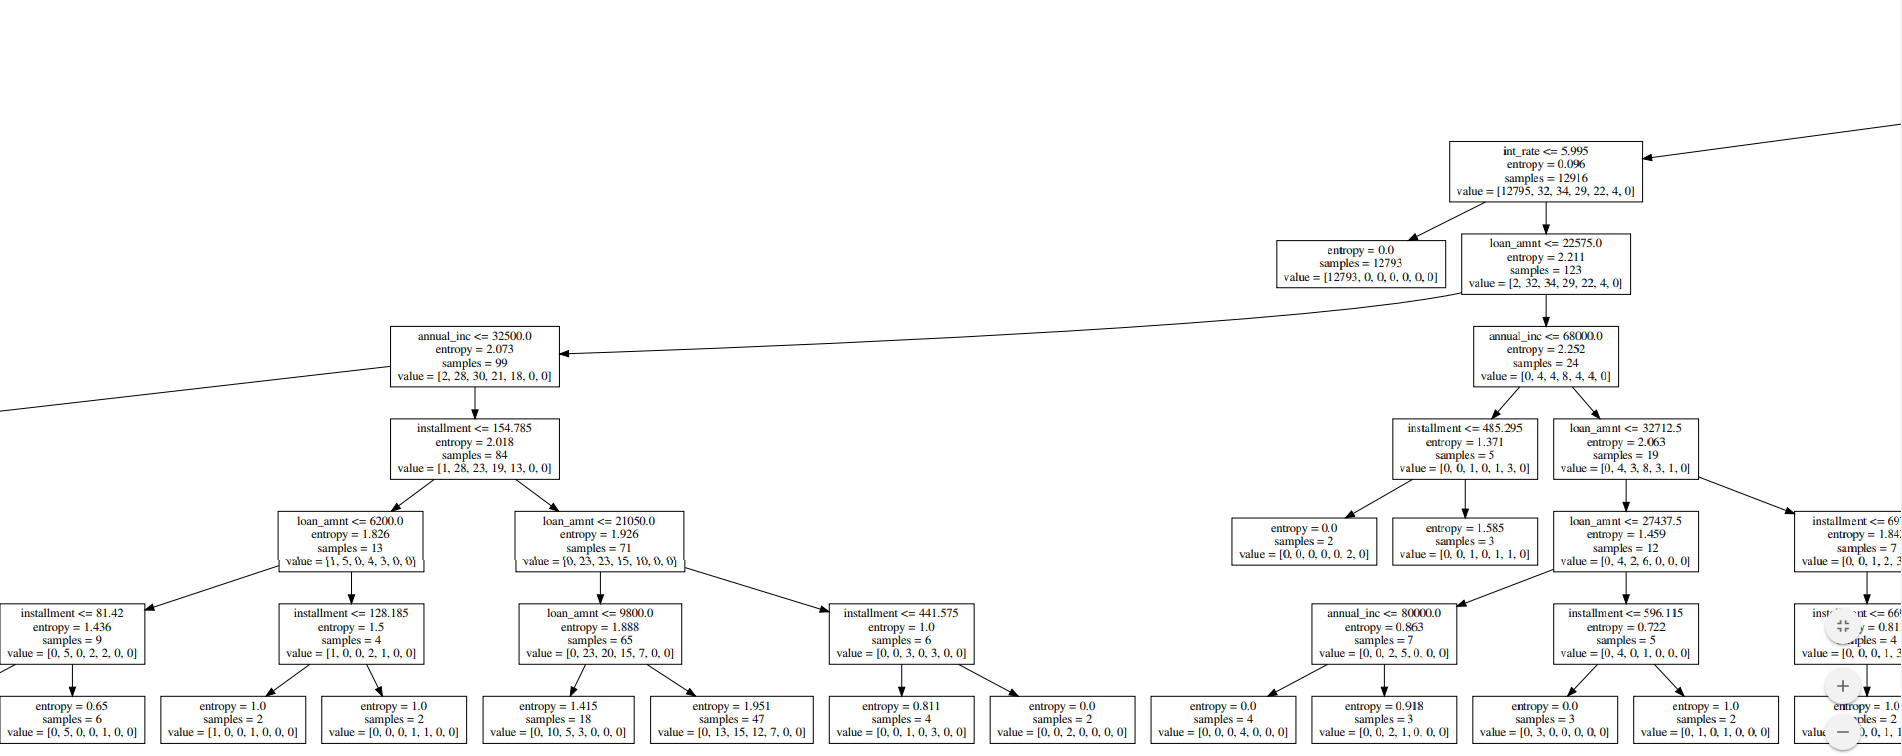
\includegraphics{34.png}
\caption{}
\end{figure}


    % Add a bibliography block to the postdoc
    
    
    
    \end{document}
